\chapter{Summarizing data}
\label{summarizingData}
\label{ch_summarizing_data}

\Comment{Do a search for "email" to see if it still appears
anywhere in this file. Do the same for the other chapters.}

\Comment{This intro was rewritten.}

This chapter focuses on the mechanics and construction
of summary statistics and graphs.
However, don't be fooled into thinking that the formulas
or graphing rules are a mathematical exercise.
These tools are applied throughout the rest of this book,
and to attain statistical excellence,
it's important to understand how these basic tools
are constructed.


%%%%%
\section[Examining numerical data]{Examining numerical data \sectionvideohref{youtube-Xm0PPtci3JE&list=PLkIselvEzpM6pZ76FD3NoCvvgkj_p-dE8}~\sectionslideshref{gdoc_os3_slides_1-6}}
\label{numericalData}

% library(openintro); ind <- c(1:5, 50); d <- loan50$interest_rate; (m <- round(mean(d), 2)); d[ind]; (dev <- d - m)[ind]; (dev2 <- dev^2)[ind]; (s2 <- sum(dev2) / 49); (s <- sqrt(s2)); var(d); sd(d); median(d); IQR(d); quantile(d, c(0.25, 0.75))
\newcommand{\loanA}{10.90}
\newcommand{\loanB}{9.92}
\newcommand{\loanC}{26.30}
\newcommand{\loanD}{9.92}
\newcommand{\loanY}{9.43}
\newcommand{\loanZ}{6.08}
\newcommand{\loanAvg}{11.57}
\newcommand{\loanVar}{25.52}
\newcommand{\loanSD}{5.05}
\newcommand{\loanN}{50}
\newcommand{\loanMedianBelow}{9.93}
\newcommand{\loanMedianAbove}{9.93}
\newcommand{\loanMedian}{9.93}
\newcommand{\loanQA}{7.96}
\newcommand{\loanQC}{13.72}
\newcommand{\loanIQR}{5.76}
\newcommand{\loanAdev}{-0.67}
\newcommand{\loanBdev}{-1.65}
\newcommand{\loanCdev}{14.73}
\newcommand{\loanDdev}{-1.65}
\newcommand{\loanYdev}{-2.14}
\newcommand{\loanZdev}{-5.49}
\newcommand{\loanSmallestValue}{5.31}
\newcommand{\loanLargestValue}{26.30}



In this section we will explore techniques for
summarizing numerical variables.
The \data{loan50} and \data{county} data sets from
Section~\ref{dataBasics} provide rich opportunities
for examples.
\Comment{Figures~\ref{} and~\ref{} show example entries of the
variables that we'll consider from those tables along
with a reminder on what each variable represents.}
If you'd like to refresh yourself on these two data
sets, see pages~\pageref{loan50DF} and~\pageref{countyDF}.
Recall that outcomes of numerical variables are numbers
on which it is reasonable to perform basic arithmetic
operations.
For example, consider the
\var{loan\_\hspace{0.3mm}amount} variable
from the \data{loan50} data set,
which represents the loan size for all 50 loans
in the data set.
This variable is numerical since we can sensibly discuss
the numerical difference of the size of two loans.
On the other hand, area codes and zip codes are not numerical,
but rather they are categorical variables.


\subsection{Scatterplots for paired data}
\label{scatterPlots}

\index{data!loan50|(}

A \term{scatterplot} provides a case-by-case view of data
for two numerical variables.
In Figure~\vref{multiunitsVsOwnership} on
page~\pageref{multiunitsVsOwnership}, a scatterplot
was used to examine the homeownership rate against
the fraction of housing units that were part of
multi-unit properties
(e.g. apartments) in the \data{county} data set.
Another scatterplot is shown in Figure~\ref{loan50_amt_vs_income},
comparing the total income of a borrower
(\var{total\_\hspace{0.3mm}income}) and the amount they borrowed
(\var{loan\_\hspace{0.3mm}amount}) for the \data{loan50} data set.
In any scatterplot, each point represents a single case.
Since there are \loanN{} cases in \data{loan50},
there are \loanN{} points in Figure~\ref{loan50_amt_vs_income}.

%\textC{\setlength{\captionwidth}{0.9\textwidth}}

\begin{figure}[h]
   \centering
   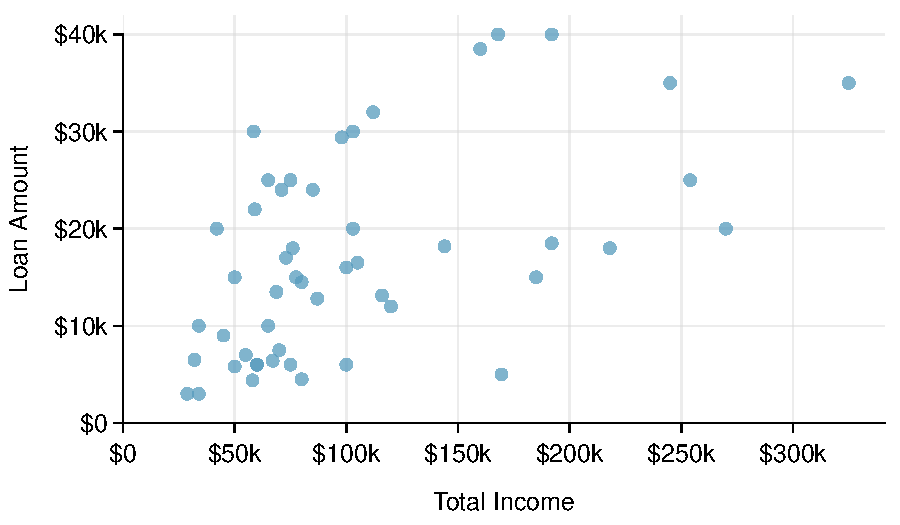
\includegraphics[width=0.8\textwidth]{ch_summarizing_data/figures/loan50_amt_vs_income/loan50_amt_vs_income}
   \caption{A scatterplot of \var{total\_\hspace{0.3mm}income}
       versus \var{loan\_\hspace{0.3mm}amount} for the
       \data{loan50} data set.}
   \label{loan50_amt_vs_income}
\end{figure}

%\textC{\setlength{\captionwidth}{\mycaptionwidth}}

Looking at Figure~\ref{loan50_amt_vs_income},
we see that there are many borrowers with an income below
\$100,000 on the left side of the graph,
while there are a handful of borrowers with income above~\$250,000.
%Additionally, the relationship appears to be \term{nonlinear},
%where bigger loans seem to be associated with increased income,
%but that it appears to taper off,
%as shown by the dashed line.

\begin{example}{Figure~\ref{medianHHIncomePoverty}
    shows a plot of median household income
    against the poverty rate for 3,143 counties.
    What can be said about the relationship between
    these variables?}
  The relationship is evidently \term{nonlinear},
  as highlighted by the dashed line.
  This is different from previous scatterplots we've seen,
  which show relationships that do not show much, if any,
  curvature in the trend.
\end{example}

\begin{figure}[h]
   \centering
   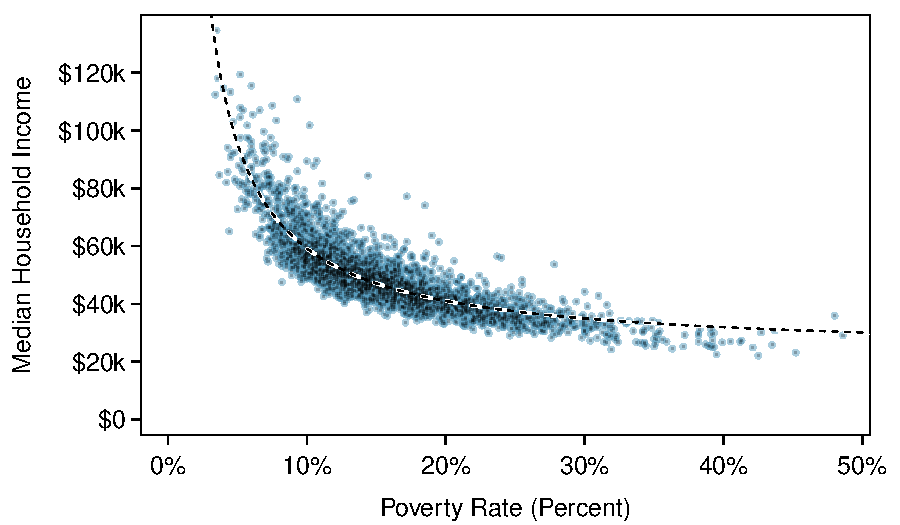
\includegraphics[width=0.8\textwidth]{ch_summarizing_data/figures/medianHHIncomePoverty/medianHHIncomePoverty}
   \caption{A scatterplot of the median household income
       against the poverty rate for the
       \data{county} data set.
       A statistical model has also been fit to the data
       and is shown as a dashed line.}
   \label{medianHHIncomePoverty}
\end{figure}

\begin{exercise}
What do scatterplots reveal about the data,
and how are they useful?\footnote{Answers may vary.
Scatterplots are helpful in quickly spotting associations
relating variables,
whether those associations come in the form of simple
trends or whether those relationships are more complex.}
\end{exercise}

%This is different from previous scatterplots we've seen, such as Figure~\vref{county_fed_spendVsPoverty} and Figure~\ref{email50LinesCharacters}, which show relationships that are very linear.

%\begin{figure}[h]
%   \centering
%   \includegraphics[width=0.8\textwidth]{ch_summarizing_data/figures/carsPriceVsWeight/carsPriceVsWeight}
%   \caption{A scatterplot of \var{price} versus \var{weight} for 54 cars.}
%   \label{carsPriceVsWeight}
%\end{figure}

\begin{exercise}
Describe two variables that would have a horseshoe-shaped
association in a scatterplot.\footnote{Consider the case
  where your vertical axis represents something ``good'' and
  your horizontal axis represents something that is only good
  in moderation.
  Health and water consumption fit this description: we require
  some water to survive, but consume too much and it becomes
  toxic and can kill a person.}
\end{exercise}

\subsection{Dot plots and the mean}
\label{dotPlot}

Sometimes two variables are one too many:
only one variable may be of interest.
In these cases, a dot plot provides the most basic of displays.
A~\term{dot plot} is a one-variable scatterplot;
an example using the interest rate of \loanN{} loans
is shown in Figure~\ref{loan_int_rate_dot_plot}.
A stacked version of this dot plot is shown in
Figure~\ref{loan_int_rate_dot_plot_stacked}.

\begin{figure}[h]
   \centering
   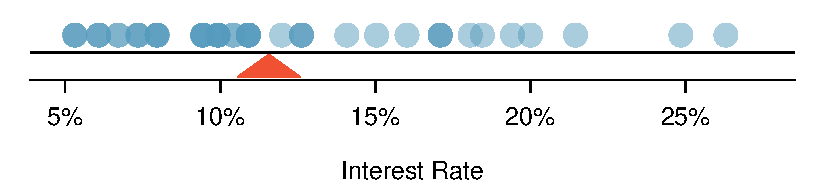
\includegraphics[width=0.76\textwidth]{ch_summarizing_data/figures/loan_int_rate_dot_plot/loan_int_rate_dot_plot}
   \caption{A dot plot of \var{interest\_\hspace{0.3mm}rate}
       for the \data{loan50} data set.
       The distribution's mean is shown as a red triangle.}
   \label{loan_int_rate_dot_plot}
\end{figure}

\begin{figure}[h]
   \centering
   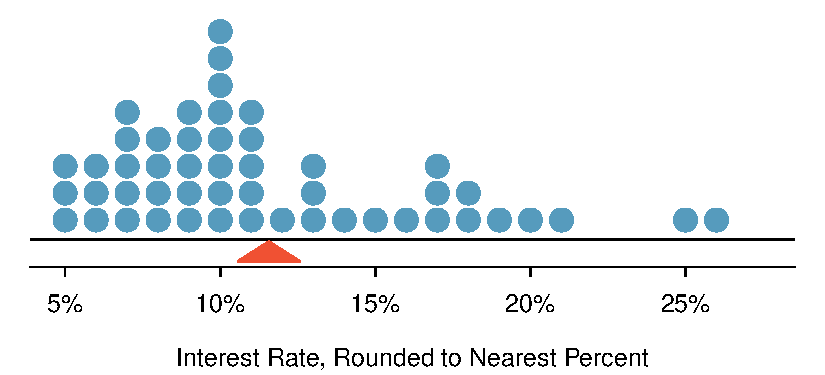
\includegraphics[width=0.76\textwidth]{ch_summarizing_data/figures/loan_int_rate_dot_plot/loan_int_rate_dot_plot_stacked}
   \caption{A stacked dot plot of
       \var{interest\_\hspace{0.3mm}rate}
       for the \data{loan50} data set.
       The~rates have been rounded to the nearest
       percent in this plot, and the
       distribution's mean is shown as a red triangle.}
   \label{loan_int_rate_dot_plot_stacked}
\end{figure}

The \term{mean}, sometimes called the
\indexthis{average}{mean!average}, is a common way
to measure the center of a \term{distribution} of data.
To compute the mean interest rate, we add up all the interest
rates and divide by the number of observations:
\begin{align*}
\bar{x}
    = \frac{\text{\loanA\%} + \text{\loanB\%} + \text{\loanC\%} +
        \cdots + \text{\loanZ\%}}{\loanN{}}
    = \loanAvg{}\%
% library(openintro); loan50$interest_rate[c(1:3, 50)]; mean(loan50$interest_rate)
\end{align*}
The sample mean is often labeled $\bar{x}$.
The letter $x$ is being used as a generic placeholder
for the variable of interest, \var{interest\_\hspace{0.3mm}rate},
and the bar over the $x$ communicates we're looking at the
average interest rate, which for these 50 loans was \loanAvg{}\%.
It is useful to think of the mean as the balancing point
of the distribution, and it is shown as a triangle in Figures~\ref{loan_int_rate_dot_plot}
and~\ref{loan_int_rate_dot_plot_stacked}.

\begin{termBox}{\tBoxTitle{Mean}%
The sample mean can be computed as the sum of the
observed values divided by the number of observations:
\begin{align*}
\bar{x} = \frac{x_1 + x_2 + \cdots + x_n}{n}
\end{align*}
where $x_1$, $x_2$, $\dots$, $x_n$ represent
the $n$ observed values.}
\end{termBox}

\begin{exercise}
Examine the equation for the mean.
What does $x_1$ correspond to? And $x_2$?
Can you infer a general meaning to what $x_i$
might represent?\footnote{$x_1$ corresponds to the
  interest rate for the first loan in the sample (\loanA\%),
  $x_2$ to the second loan's interest rate (\loanB\%),
  and $x_i$ corresponds to the interest rate for the
  $i^{th}$ loan in the data set.}
\end{exercise}

\begin{exercise}
What was $n$ in this sample of
loans?\footnote{The sample size was $n = 50$.}
\end{exercise}

The \data{loan50} data set represents a sample from
a larger population of loans made through Lending Club.
We could compute a mean for this population in the same way
as the sample mean.
However, the population mean has a special label: $\mu$.
\index{Greek!mu@mu ($\mu$)}
The symbol $\mu$ is the Greek letter \emph{mu} and represents
the average of all observations in the population.
Sometimes a subscript, such as $_x$,
is used to represent which variable the population mean
refers to, e.g. $\mu_x$.
Often times it is too expensive to measure the
population mean precisely, so we often estimate
$\mu$ using the sample mean, $\bar{x}$.

\begin{example}{The average interest rate across all loans
  in the population can be estimated using the sample data.
  Based on the sample of 50 loans,
  what would be a reasonable estimate of $\mu_x$,
  the mean interest rate for all loans in the
  full data set?}
The sample mean, \loanAvg{}\%, may provide a reasonable estimate
of $\mu_x$.
While this number will not be perfect,
it provides a \emph{point estimate} \index{point estimate}
of the average interest rate of all the loans in the
population under study.
In Chapter~\ref{foundationsForInference} and beyond,
we will develop tools to characterize the accuracy
of point estimates, and we will find that point estimates
based on larger samples tend to be more accurate than
those based on smaller samples.
\end{example}

\Comment{Next example is new and tries to highlight
\emph{why} the mean is so useful.}

The mean is useful because it allows us to
rescale or standardize a metric to something more easily
interpretable and comparable.

\begin{example}{Provide a couple examples where the mean
  is a useful tool for making comparisons.}

  1. We would like to understand if a new drug is more
  effective at treating asthma attacks than the standard
  treatment.
  A trial of 1500 adults is set up,
  where 500 receive the new drug in the treatment group,
  and 1000 receive a standard drug in the control group.
  Suppose we observe 200 asthma attacks in the treatment
  group and 300 asthma attacks in the control group.
  We cannot reasonably compare 200 to 300
  since the group sizes are different.
  However, we can control for the imbalanced group sizes
  by computing the average number of asthma attacks per
  patient in each group.
  The standard drug has a lower
  average number of asthma attacks per patient % (0.3 per patient)
  than the average in the treatment group: % (0.4 per patient).
  \begin{align*}
  & \text{Control Group: }\frac{300}{1000} = 0.3
      && \text{Treatment Group: } \frac{200}{500} = 0.4 % \\
  % &     &&  %\\
  % & = 0.3\text{ asthma attacks per patient}
  %     && = 0.4\text{ asthma attacks per patient}
  \end{align*}

  2. Emilio opened a food truck last year where he sells burritos,
  and his business has stabilized over the last 3 months.
  Over that 3 month period, he has made \$11,000 while
  working 625 hours.
  Emilio's average hourly earnings provides
  a useful statistic for evaluating whether his venture is,
  at least from a financial perspective, worth it:
  \begin{align*}
  \frac{\$11000}{625\text{ hours}} = \$17.60\text{ per hour}
  \end{align*}
  By knowing his average hourly wage,
  Emilio now has put his earnings into a standard unit that
  is easier to compare with many other jobs that he could
  apply for.
\end{example}

%\begin{example}{What are some contexts that highlight
%    the value of the mean?}
%  Here are a few scenarios highlighting why the mean can be
%  particularly useful.
%  \begin{itemize}
%  \item If a waitress makes an average of \$3.20 per table,
%      then she can get a reasonable estimate of how much
%      money she will make if she knows she'll turn over
%      about 15 tables in a night:
%      \begin{align*}
%      total &= average \times count
%          = \$3.20 \times 15
%          = \$48.00
%      \begin{align*}
%      The estimate won't be perfect, but it will still
%      be a useful reference of what she can expect.
%  \item For every \$1 played on roulette,
%      a gambler will lose, on average, 2.7 cents.
%      If she plays 1000 games and bets \$1 each time,
%      her expected loss is
%      \begin{align*}
%      total = average \times count
%          = 2.7 \cents \times 1000
%          = \$27
%      \begin{align*}
%  \end{itemize}
%  The average provides us a sensible value to think
%  about scaling gains and losses.
%\end{example}

\begin{example}{We might like to compute the average income
    per person in the US. To do so, we might first think to take
    the mean of the per capita incomes across the 3,143 counties
    in the \data{county} data set. What would be a better approach?}
    \label{wtdMeanOfIncome}
  The \data{county} data set is special in that each county
  actually represents many individual people.
  If we were to simply average across the \var{income}
  variable, we would be treating counties with 5,000 and
  5,000,000 residents equally in the calculations.
  Instead, we should compute the total income for each county,
  add up all the counties' totals, and then divide by the number
  of people in all the counties.
  If we completed these steps with the \data{county} data,
  we would find that the per capita income for the US is
  \$27,348.43.
  Had we computed the \emph{simple} mean of per capita income
  across counties, the result would have been just \$22,504.70!
\end{example}

Example~\ref{wtdMeanOfIncome} used what is called
a \term{weighted mean}\index{mean!weighted mean},
which will not be a key topic in this textbook.
However, we have provided an online supplement on
weighted means for interested readers under
\Comment{Extra Content at
\oiRedirect{os}{openintro.org/os}}.

\subsection{Histograms and shape}
\label{histogramsAndShape}

Dot plots show the exact value for each observation.
This is useful for small data sets, but they can become
hard to read with larger samples. Rather than showing the
value of each observation, we prefer to think of the value
as belonging to a \emph{bin}.
For example, in the \data{loan50} data set, we created
a table of counts for the number of loans with interest
rates between 5.0\% and 7.5\%, then the number of loans
with rates between 7.5\% and 10.0\%, and so on.
Observations that fall on the boundary of a bin
(e.g. 10.00\%) are allocated to the lower bin.
This tabulation is shown in Figure~\ref{binnedIntRateAmountTable}.
These binned counts are plotted as bars in
Figure~\ref{loan50IntRateHist} into what is called
a \term{histogram}, which resembles a more heavily binned
version of the stacked dot plot shown in
Figure~\ref{loan_int_rate_dot_plot_stacked}.

\begin{figure}[ht]
\centering\small
\begin{tabular}{l ccc ccc ccc} % c}
  \hline
  % cat(paste0(gsub(" ", "", format(a)), "\\% - ", gsub(" ", "", format(b)), "\\%", collapse = " & "))
  % cat(paste0(gsub(" ", "", format(a)), "-", gsub(" ", "", format(b)), collapse = " & "))
Interest Rate & 5.0\% - 7.5\% & 7.5\% - 10.0\% & 10.0\% - 12.5\% & 12.5\% - 15.0\% & $\cdots$ & 25.0\% - 27.5\% \\
%in \$1000's & \raisebox{1.5ex}[0pt]{0-5} & \raisebox{1.5ex}[0pt]{5-10} & \raisebox{1.5ex}[0pt]{10-15} & \raisebox{1.5ex}[0pt]{15-20} & \raisebox{1.5ex}[0pt]{20-25} & \raisebox{1.5ex}[0pt]{25-30} & \raisebox{1.5ex}[0pt]{30-35} & \raisebox{1.5ex}[0pt]{35-40} \\
  \hline
Count & 11 &  15 &   8 &   4 &   $\cdots$ &   1 \\
  \hline
\end{tabular}
\caption{Counts for the binned
    \var{interest\_\hspace{0.3mm}rate} data.}
\label{binnedIntRateAmountTable}
\end{figure}
% library(openintro); library(xtable); d <- loan50$interest_rate; max(d); t1 <- table(cut(d, seq(5, 27.5, 2.5), right = TRUE)); t1; xtable(rbind(t1))

\begin{figure}[bth]
   \centering
   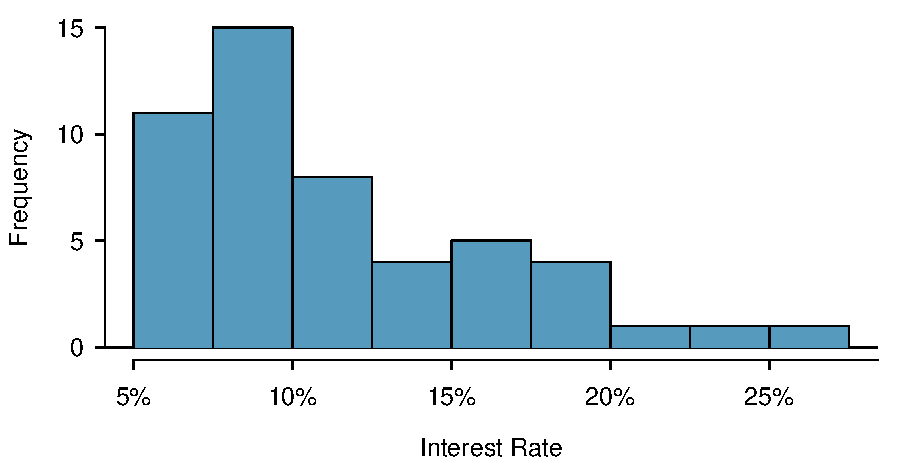
\includegraphics[width=0.82\textwidth]{ch_summarizing_data/figures/loan50IntRateHist/loan50IntRateHist}
   \caption{A histogram of \var{num\_\hspace{0.3mm}char}. This distribution is very strongly skewed to the right.\index{skew!example: very strong}}
   \label{loan50IntRateHist}
\end{figure}

Histograms provide a view of the \term{data density}.
Higher bars represent where the data are relatively more common.
For instance, there are many more loans with rates between
5\%~and~10\% than loans with rates between 20\% and~25\%
in the data set.
The bars make it easy to see how the density of the data
changes relative to the number of characters.

Histograms are especially convenient for describing the
shape of the data distribution\label{shapeFirstDiscussed}.
Figure~\ref{loan50IntRateHist} suggests that most loans
have rates under 15\%, while only a handful
of loans have rates above 20\%.
When data trail off to the right in this way
and has a longer right \hiddenterm{tail}\index{skew!tail},
the shape is said to be
\termsub{right skewed}{skew!right skewed}.\footnote{Other
  ways to describe data that are skewed to the right:
  \termni{skewed to the right},
  \termni{skewed to the high end},
  or \termni{skewed to the positive end}.}

Data sets with the reverse characteristic --
a long, thinner tail to the left --
are said to be \termsub{left skewed}{skew!left skewed}.
We also say that such a distribution has a long left tail.
Data sets that show roughly equal trailing off in both
directions are called \term{symmetric}.\index{skew!symmetric}

\begin{termBox}{\tBoxTitle{Long tails to identify skew}%
  When data trail off in one direction, the distribution
  has a \term{long tail}. \index{skew!long tail|textbf}
  If a distribution has a long left tail, it is left skewed.
  If a distribution has a long right tail, it is right skewed.}
\end{termBox}

\begin{exercise}
Take a look at the dot plots in
Figures~\ref{loan_int_rate_dot_plot}
and~\ref{loan_int_rate_dot_plot_stacked}.
Can you see the skew in the data? Is it easier to see the
skew in this histogram or the dot plots?\footnote{The skew
  is visible in all three plots, though the flat dot plot
  is the least useful.
  The stacked dot plot and histogram are helpful
  visualizations for identifying skew.}
\end{exercise}

\begin{exercise}
Besides the mean (since it was labeled), what can you see
in the dot plots that you cannot see in the
histogram?\footnote{The interest rates for individual loans.}
\end{exercise}

In addition to looking at whether a distribution is skewed
or symmetric, histograms can be used to identify modes.
A \term{mode} is represented by a prominent peak in the
distribution.\footnote{A definition of \emph{mode} sometimes
  taught in math classes is the value with the
  most occurrences in the data set.
  However, for many real-world data sets, it is common to have
  \emph{no} observations with the same value in a data set,
  making this definition less practical in data analysis.}
There is only one prominent peak in the histogram of
\var{loan\_\hspace{0.3mm}amount}.

Figure~\ref{singleBiMultiModalPlots} shows histograms that
have one, two, or three prominent peaks.
Such distributions are called
\termsub{unimodal}{modality!unimodal},
\termsub{bimodal}{modality!bimodal}, and
\termsub{multimodal}{modality!multimodal}, respectively.
Any distribution with more than 2~prominent peaks is
called multimodal.
Notice that there was one prominent peak in the unimodal
distribution with a second less prominent peak that was
not counted since it only differs from its neighboring
bins by a few observations.

\begin{figure}[h]
   \centering
   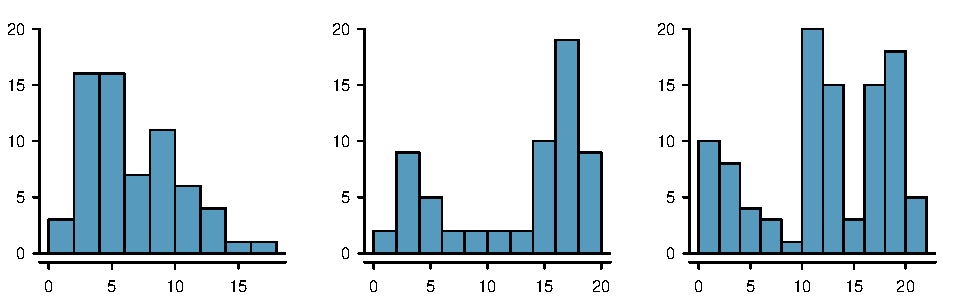
\includegraphics[width=0.98\textwidth]{ch_summarizing_data/figures/singleBiMultiModalPlots/singleBiMultiModalPlots}
   \caption{Counting only prominent peaks, the distributions are (left to right) unimodal, bimodal, and multimodal. Note that we've said the left plot is unimodal intentionally. This is because we are counting \emph{prominent} peaks, not just any peak. See the Tip box for more thoughts.}
   \label{singleBiMultiModalPlots}
\end{figure}

\begin{example}{Figure~\ref{loan50IntRateHist}
    reveals only one prominent mode in the interest rate.
    Is the distribution unimodal, bimodal, or multimodal?}
  Unimodal.
  Remember that \emph{uni} stands for 1 (think \emph{uni}cycles).
  Similarly, \emph{bi} stands for~2 (think \emph{bi}cycles).
  (We're hoping a \emph{multicycle} will be invented to complete
  this analogy.)
\end{example}

%\begin{example}{Looking back the stacked dot plot in
%    Figure~\ref{loan_int_rate_dot_plot_stacked},
%    it would be reasonable to wonder if the distribution
%    of loan amounts is actually bimodal or even multimodal.
%    In fact, we wondered the same thing -- so we investigated!}
%  What we found is that the bumps evident in the dot plot
%  tend to happen at \$5,000 increments.
%  That is, people made loan requests in round amounts.
%  While that is interesting, we often are more interested
%  in understanding the general shape of a data set rather
%  than characterizing some special property like this,
%  and for this reason, we think the data set is better
%  described as unimodal.
%  However, this example highlights that there isn't
%  always one ``correct'' answer for the number of modes.
%
%  There's a broader lesson to take away
%  from this example:
%  when we plot data in multiple ways,
%  we learn about different properties of the data
%  that no one plot would reveal all on its own.
%\end{example}

\begin{exercise}
Height measurements of young students and adult teachers
at a K-3 elementary school were taken.
How many modes would you expect in this height data
set?\footnote{There might be two height groups visible
  in the data set: one of the students and one of the adults.
  That is, the data are probably bimodal.}
\end{exercise}

Looking for modes isn't about finding a clear and correct
answer about the number of modes in a distribution,
which is why \emph{prominent}\index{prominent} is not
rigorously defined in this book.
The important part of this examination is to better
understand your data.



\subsection{Variance and standard deviation}
\label{variability}

The mean was introduced as a method to describe the center of a data set, and \indexthis{variability}{variability} in the data is also important. Here, we introduce two measures of variability: the variance and the standard deviation. Both of these are very useful in data analysis, even though their formulas are a bit tedious to calculate by hand. The standard deviation is the easier of the two to understand, and it roughly describes how far away the typical observation is from the mean.

We call the distance of an observation from its mean its \term{deviation}. Below are the deviations for the $1^{st}_{}$, $2^{nd}_{}$, $3^{rd}$, and $50^{th}_{}$ observations in the \var{loan\_\hspace{0.3mm}amount} variable.
For computational convenience, we'll perform the calculations
in thousands of dollars rounded to the nearest \$100:
\begin{align*}
x_1^{}-\bar{x} &= \loanA - \loanAvg{} = \loanAdev \hspace{5mm}\text{ } \\
x_2^{}-\bar{x} &= \loanB - \loanAvg{} = \loanBdev \\
x_3^{}-\bar{x} &= \loanC - \loanAvg{} = \loanCdev \\
			&\ \vdots \\
x_{50}^{}-\bar{x} &= \loanZ - \loanAvg{} = \loanZdev
\end{align*}
\Comment{Next sentence says ``average'' even though
  it is dividing by $n - 1$.
  Same change in the term box below. Thoughts?}
If we square these deviations and then take an average,
the result is equal to the sample
\term{variance}\label{varianceIsDefined},
denoted by $s_{}^2$:
\begin{align*}
s_{}^2 &= \frac{(\loanAdev)_{}^2 + (\loanBdev)_{}^2 + (\loanCdev)_{}^2 + \cdots + (\loanZdev)_{}^2}{\loanN{}-1} \\
	&= \frac{0.45 + 2.72 + 216.97 + \cdots + 30.14}{49} \\
	&= \loanVar{}
\end{align*}
We divide by $n - 1$, rather than dividing by $n$,
when computing the variance;
you need not worry about this mathematical nuance
for the material in this textbook.
Notice that squaring the deviations does two things.
First, it makes large values relatively much larger,
seen by comparing $(\loanAdev)^2$, $(\loanBdev)^2$, $(\loanCdev)^2$,
and $(\loanZdev)^2$.
Second, it gets rid of any negative signs.

The \term{standard deviation} is defined as the square root of the variance:
\begin{align*}
s = \sqrt{\loanVar{}} = \loanSD{}
\end{align*}
A subscript of $_x$ may be added to the variance
and standard deviation,
i.e. $s_x^2$ and $s_x^{}$, as a reminder that these
are the variance and standard deviation of the observations
represented by $x_1^{}$, $x_2^{}$, ..., $x_n^{}$.
The $_{x}$ subscript is usually omitted when it is clear
which data is being referenced.

\begin{termBox}{\tBoxTitle{Variance and standard deviation}
  The variance is the average squared distance from the mean.
  The standard deviation is the square root of the variance.
  The standard deviation is useful when considering how far
  the data are distributed from the mean.}
\end{termBox}

\Comment{This paragraph has been shortened to focus
  exclusively on the notation for the population and
  omits the $n - 1$ and $n$ distinction.}
%The formula for computing a population's variance
%and standard deviation are similar
%to those used for a sample.\footnote{The only difference
%  is that the population variance has a division by $n$
%  instead of $n-1$.}
%However, like the mean, the population values have
%special symbols:
%$\sigma_{}^2$ for the variance and $\sigma$ for the
%standard deviation.
%The symbol $\sigma$ \index{Greek!sigma@sigma ($\sigma$)}
%is the Greek letter \emph{sigma}.
Like the mean, the population values for variance
and standard deviation have special symbols:
$\sigma_{}^2$ for the variance and $\sigma$ for the
standard deviation.
The symbol $\sigma$ \index{Greek!sigma@sigma ($\sigma$)}
is the Greek letter \emph{sigma}.

\begin{figure}
\centering
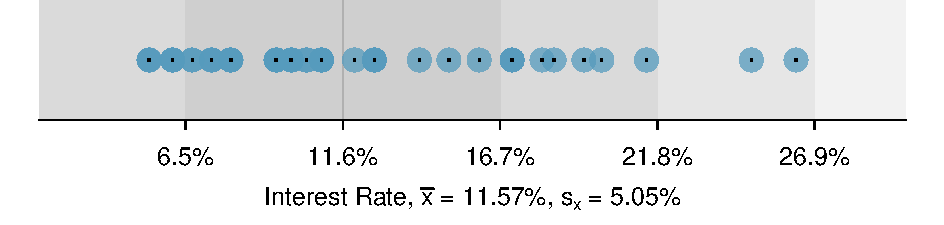
\includegraphics[width=\mycaptionwidth]{ch_summarizing_data/figures/sdRuleForIntRate/sdRuleForIntRate}
\caption{For the \var{interest\_\hspace{0.3mm}rate} variable,
  34 of the 50 loans (68\%) had interest rates within
  1~standard deviation of the mean,
  and 48 of the 50 loans (96\%) had rates within
  2~standard deviations.
  Usually about 70\% of the data are within 1~standard
  deviation of the mean and 95\% within 2~standard
  deviations, though this is far from a hard rule.}
\label{sdRuleForIntRate}
\end{figure}

\Comment{The following box was changed from a Tip Box
  to a Term Box since the design of OS4 will not distinguish
  between the two.
  The title was also updated}

\begin{termBox}{
  \tBoxTitle{How to think about the standard deviation}
  The standard deviation represents the typical deviation
  of observations from the mean.
  Usually about 70\% of the data will be within one standard
  deviation of the mean and about 95\% will be within two
  standard deviations.
  However, as seen in Figures~\ref{sdRuleForLoanAmount}
  and~\ref{severalDiffDistWithSdOf1}, these percentages are
  not strict rules.}
\end{termBox}

\begin{figure}
\centering
\includegraphics[width=0.64\textwidth]{ch_summarizing_data/figures/severalDiffDistWithSdOf1/severalDiffDistWithSdOf1}
\caption{Three very different population distributions
  with the same mean $\mu=0$ and standard deviation $\sigma=1$.}
\label{severalDiffDistWithSdOf1}
\end{figure}

\begin{exercise}
On page~\pageref{shapeFirstDiscussed}, the concept of
shape of a distribution was introduced.
A good description of the shape of a distribution should
include modality and whether the distribution is symmetric
or skewed to one side.
Using Figure~\ref{severalDiffDistWithSdOf1} as an example,
explain why such a description is
important.\footnote{Figure~\ref{severalDiffDistWithSdOf1}
  shows three distributions that look quite different,
  but all have the same mean, variance,
  and standard deviation.
  Using modality, we can distinguish between the
  first plot (bimodal) and the last two (unimodal).
  Using skewness, we can distinguish between the
  last plot (right skewed) and the first two.
  While a picture, like a histogram, tells a more
  complete story, we can use modality and shape
  (symmetry/skew) to characterize basic information
  about a~distribution.}
\end{exercise}

\begin{example}{Describe the distribution of the
    \var{interest\_\hspace{0.3mm}rate} variable using
    the histogram in Figure~\ref{loan50IntRateHist}.
    The description should incorporate the center,
    variability, and shape of the distribution,
    and it should also be placed in context.
    Also note any especially unusual cases.}
  The distribution of interest rates is unimodal
  and skewed to the high end.
  Many of the rates fall near the mean at 11.57\%,
  and most fall within one standard deviation (5.05\%)
  of the mean.
  There are a few exceptionally large interest rates
  in the sample that are above 20\%.
\end{example}

In practice, the variance and standard deviation are sometimes
used as a means to an end, where the ``end'' is being able to
accurately estimate the uncertainty associated with a sample
statistic.
For example, in Chapter~\ref{foundationsForInference}
the standard deviation is used in calculations that help us
understand how much a sample mean varies from one sample
to the next.


\subsection{Box plots, quartiles, and the median}

A \term{box plot} summarizes a data set using five
statistics while also plotting unusual observations.
Figure~\ref{loan_int_rate_box_plot_layout} provides
a vertical dot plot alongside a box plot of the
\var{interest\_\hspace{0.3mm}rate} variable from
the \data{loan50} data set.

\begin{figure}[h]
   \centering
   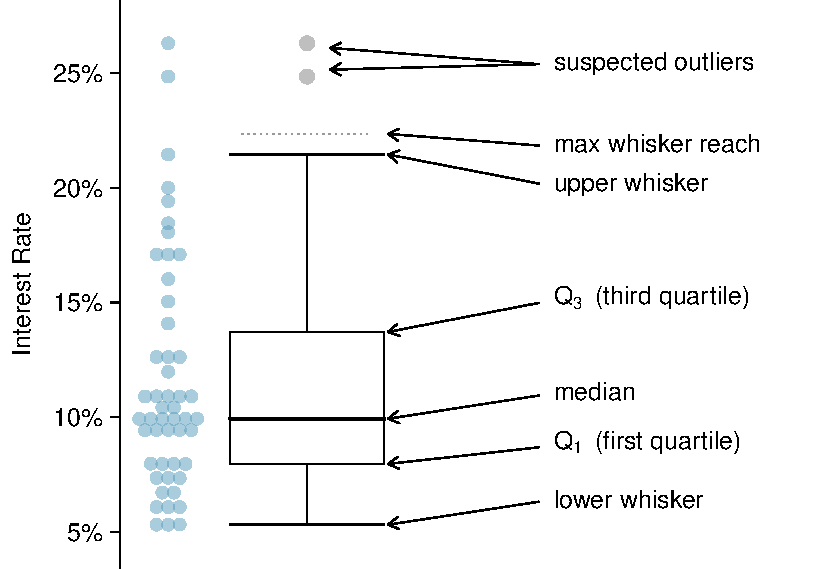
\includegraphics[width=0.86\mycaptionwidth]{ch_summarizing_data/figures/loan_int_rate_box_plot_layout/loan_int_rate_box_plot_layout}
   \caption{A vertical dot plot next to a labeled box plot
       for the interest rates of the \loanN{} loans.
       The median (\loanMedian{}), splits the data into the
       bottom 50\% and the top 50\%.}
   \label{loan_int_rate_box_plot_layout}
\end{figure}

The first step in building a box plot is drawing a dark line
denoting the \term{median}, which splits the data in half.
Figure~\ref{loan_int_rate_box_plot_layout} shows 50\% of the
data falling below the median and other 50\% falling above
the median.
There are \loanN{} character counts in the data set
(an even number) so the data are perfectly split into two
groups of~25.
We take the median in this case to be the average of the
two observations closest to the $50^{th}$ percentile,
which happen to be the same value in this data set:
$(\text{\loanMedianAbove{}} + \text{\loanMedianBelow{}}) / 2
  = \text{\loanMedian{}}$.
When there are an odd number of observations,
there will be exactly one observation that splits the data
into two halves, and in such a case that observation
is the median (no average needed).

\begin{termBox}{\tBoxTitle{Median: the number in the middle}
  If the data are ordered from smallest to largest,
  the \term{median} is the observation right in the middle.
  If there are an even number of observations,
  there will be two values in the middle,
  and the median is taken as their average.}
\end{termBox}

The second step in building a box plot is drawing
a rectangle to represent the middle 50\% of the data.
The total length of the box, shown vertically in
Figure~\ref{loan_int_rate_box_plot_layout},
is called the \term{interquartile range} (\hiddenterm{IQR},
for short).
It, like the standard deviation, is a measure
of \indexthis{variability}{variability} in data.
The more variable the data, the larger the standard
deviation and~IQR tend to be.
The two boundaries of the box are called the
\term{first quartile} \index{quartile!first quartile}
(the $25^{th}$ \hiddenterm{percentile},
i.e. 25\% of the data fall below this value)
and the \term{third quartile} \index{quartile!third quartile}
(the $75^{th}$ percentile), and these are often labeled $Q_1$
\index{Q$_1$} and $Q_3$\index{Q$_3$}, respectively.

\begin{termBox}{\tBoxTitle{Interquartile range (IQR)}
  The IQR\index{interquartile range} is the length
  of the box in a box plot.
  It is computed as
  \begin{eqnarray*}
  IQR = Q_3 - Q_1
  \end{eqnarray*}
  where $Q_1$ and $Q_3$ are the $25^{th}$ and $75^{th}$
  percentiles.}
\end{termBox}

\begin{exercise}
What percent of the data fall between $Q_1$ and the median?
What percent is between the median and $Q_3$?\footnote{Since
  $Q_1$ and $Q_3$ capture the middle 50\% of the data and
  the median splits the data in the middle, 25\% of the data
  fall between $Q_1$ and the median, and another 25\% falls
  between the median and $Q_3$.}
\end{exercise}

Extending out from the box, the \term{whiskers} attempt
to capture the data outside of the box.
However, their reach is never allowed to be more than
$1.5\times IQR$.
They capture everything within this reach.
In Figure~\ref{loan_int_rate_box_plot_layout},
the upper whisker does not extend to the last two points,
which is beyond $Q_3 + 1.5\times IQR$,
and so it extends only to the last point below this limit.
The lower whisker stops at the lowest value,
\loanSmallestValue{}\%,
since there is no additional data to reach;
the lower whisker's limit is not shown in the figure because
the plot does not extend down to $Q_1 - 1.5\times IQR$.
In a sense, the box is like the body of the box plot
and the whiskers are like its arms trying to reach the
rest of the data.

Any observation lying beyond the whiskers is labeled with a dot.
The purpose of labeling these points --
instead of extending the whiskers to the minimum
and maximum observed values --
is to help identify any observations that appear to be
unusually distant from the rest of the data.
Unusually distant observations are called
\termsub{outliers}{outlier}.
In this case, it would be reasonable to classify the
interest rates of 24.85\% and \loanLargestValue{}\%
as outliers since they are numerically distant from
most of the data.

\begin{termBox}{\tBoxTitle{Outliers are extreme}
  An \term{outlier} is an observation that appears
  extreme relative to the rest of the data. \vspace{3mm}
  
  Examining data for outliers serves
  many useful purposes, including\vspace{-1mm}
  \begin{enumerate}
  \setlength{\itemsep}{0mm}
  \item Identifying
      \indexthis{strong skew}{skew!example: strong}
      in the distribution.
  \item Identifying possible data collection or entry
      errors.
  \item Providing insight into interesting properties
      of the data.\vspace{-1mm}
  \end{enumerate}}
\end{termBox}

%\begin{exercise}
%The observation \loanLargestValue{}\%, a suspected outlier,
%was found to be an accurate observation.
%What would such an observation suggest about the nature
%of interest rates through Lending Club?\footnote{That
%  occasionally there may be very long emails.}
%\end{exercise}

\begin{exercise}
Using Figure~\ref{loan_int_rate_box_plot_layout},
estimate the following values for
\var{interest\_\hspace{0.3mm}rate} in the
\data{loan50} data set:
(a) $Q_1$,
(b) $Q_3$, and
(c) IQR.\footnote{These
  visual estimates will vary a little from one person
  to the next:
  $Q_1=$ 8\%,
  $Q_3=$ 14\%,
  $\text{IQR} = Q_3 - Q_1 = 6\%$.
  (The true values: $Q_1= \loanQA{}\%$, $Q_3 = \loanQC{}\%$,
  $\text{IQR} = \loanIQR{}\%$.)}
\end{exercise}

\CalculatorVideos{how to create statistical summaries and box plots}


\subsection{Robust statistics}

How are the \indexthis{sample statistics}{sample statistic}
of the \data{interest\_\hspace{0.3mm}rate} data set affected
by the observation, 26.30\%?
What would have happened if this loan had instead
been only 15.00\%?
What would happen to these
\indexthis{summary statistics}{summary statistic}
if the observation at 26.30\% had been even larger,
say 35.00\%? These scenarios are plotted alongside the
original data in Figure~\ref{loan_int_rate_robust_ex},
and sample statistics are computed under each scenario in
Figure~\ref{robustOrNotTable}.

\begin{figure}[ht]
\centering
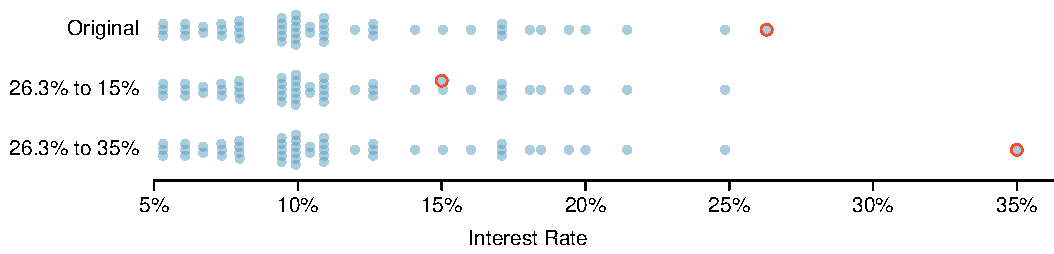
\includegraphics[width=\textwidth]{ch_summarizing_data/figures/loan_int_rate_robust_ex/loan_int_rate_robust_ex}
\caption{Dot plots of the original interest rate data
  and two modified data sets.}
\label{loan_int_rate_robust_ex}
\end{figure}

% See `loan_int_rate_robust_ex` figure code for calculations.
\begin{figure}[ht]
\centering
\begin{tabular}{l c cc c cc}
% \cline{3-4} \cline{6-7}
& \hspace{0mm} & \multicolumn{2}{c}{\bf robust} &
    \hspace{2mm} & \multicolumn{2}{c}{\bf not robust} \\
\hline
scenario && median & IQR && $\bar{x}$ & $s$ \\ 
\hline
%   & & \multicolumn{2}{c|} & & \multicolumn{2}{c|} \\
original \var{num\_\hspace{0.3mm}char} data
    && 9.93\% & 5.76\% && 11.57\% & 5.05\% \\
move 26.30\% $\to$ 15.00\%
    && 9.93\% & 5.76\% && 11.34\% & 4.61\% \\
move 26.30\% $\to$ 35.00\%
    && 9.93\% & 5.76\% && 11.74\% & 5.68\% \\
   \hline
\end{tabular}
\caption{A comparison of how the median, IQR,
  mean ($\bar{x}$), and standard deviation ($s$) change
  when an extreme observations is shifted.}
\label{robustOrNotTable}
\end{figure}

\begin{exercise} \label{interestRateWhichIsMoreRobust}
(a)~Which is more affected by extreme observations,
the mean or median?
Figure~\ref{robustOrNotTable} may be helpful.
(b)~Is the standard deviation or IQR more affected by
extreme observations?\footnote{(a)~Mean is affected more.
(b)~Standard deviation is affected more.
  Complete explanations are provided in the material
  following Guided Practice~\ref{interestRateWhichIsMoreRobust}.}
\end{exercise}

The median and IQR are called \term{robust statistics} because
extreme observations have little effect on their values:
moving the most extreme value generally has little influence
on these statistics.
On the other hand, the mean and standard deviation
are more heavily influenced by changes in extreme observations.

\begin{example}{The median and IQR did not change under the
    three scenarios in Figure~\ref{robustOrNotTable}.
    Why might this be the case?}
  The median and IQR are only sensitive to numbers
  near $Q_1$, the median, and $Q_3$.
  Since values in these regions are stable in the three
  data sets, the median and IQR estimates are also stable.
\end{example}

\Comment{The next exercise hits on one possible distinction
  between median / mean: use the median if we care about
  understanding the typical individual case.
  However, if we care about something that scales
  or will be more impactful to a full business,
  then the mean is probably more useful.}

\begin{exercise}
The distribution of loan amounts in \data{loan50}
is right skewed, with a few large loans lingering
out into the right tail.
If you were wanting to understand the typical loan size,
should you be more interested in the mean
or median?\footnote{Answers will vary!
  If looking to simply understand what a typical individual
  loan looks like, the median is probably more useful.
  However, if the goal is to understand something that
  scales well, such as the total amount of money we might
  need to have on hand if we were to offer 1,000 loans,
  then the mean would be more useful.}
\end{exercise}

\index{data!loan50|)}


\subsection{Transforming data (special topic)}
\label{transformingDataSubsection}

When data are very strongly skewed, we sometimes transform
them so they are easier to model.

\begin{figure}[ht]
\centering
\subfigure[]{
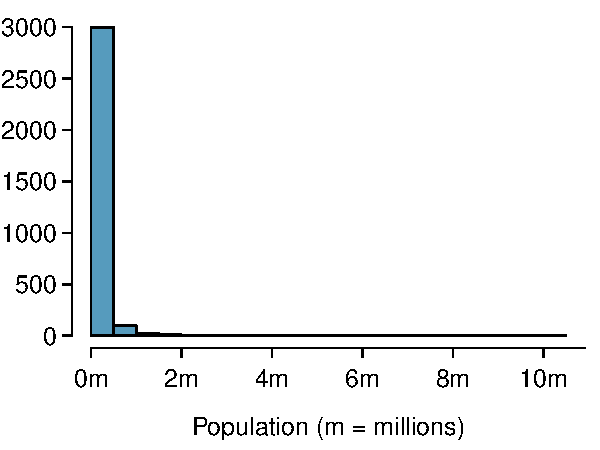
\includegraphics[width=0.46\textwidth]{ch_summarizing_data/figures/county_pop_transformed/county_pop_transformed_i}
\label{county_pop_transformed_i}
}
\subfigure[]{
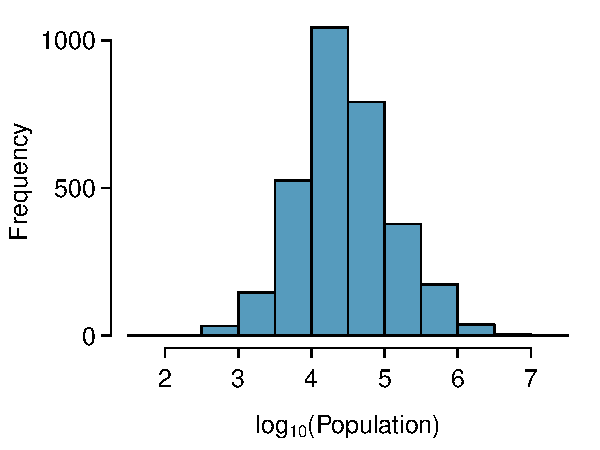
\includegraphics[width=0.46\textwidth]{ch_summarizing_data/figures/county_pop_transformed/county_pop_transformed_log}
\label{county_pop_transformed_log}
}
\caption{\subref{county_pop_transformed_i} A histogram of
  the populations of all US counties.
  \subref{county_pop_transformed_log} A histogram of
  log$_{10}$-transformed county populations.
  For this plot, the x-value corresponds to the power
  of 10, e.g. ``4'' on the x-axis corresponds to $10^4 =$ 10,000.}
\label{county_pop_transformed}
\end{figure}

\begin{example}{Consider the histogram of county populations
    shown in Figure~\ref{county_pop_transformed_i},
    which shows extreme skew\index{skew!example: extreme}.
    What isn't useful about this plot?}
  Nearly all of the data fall into the left-most bin,
  and the extreme skew obscures many of the potentially
  interesting details in the data.
\end{example}

There are some standard transformations that may be
useful for strongly right skewed data where much of the
data is positive but clustered near zero.
A \term{transformation} is a rescaling of the data
using a function.
For instance, a plot of the logarithm (base 10) of
county populations results in the new histogram in
Figure~\ref{county_pop_transformed_log}.
This data is symmetric, and any potential outliers
appear much less extreme than in the original data set.
By reigning in the outliers and extreme skew,
transformations like this often make it easier to build
statistical models against the data.

Transformations can also be applied to one or both
variables in a scatterplot.
A scatterplot of the the population change from 2010 to 2017
against the population in 2010 is shown in Figure~\ref{county_pop_change_v_pop_transform_i}.
In this first scatterplot, it's hard to decipher any
interesting patterns because the population variable
is so strongly skewed.
However, if we apply a log$_{10}$ transformation to
the population variable, as shown in
Figure~\ref{county_pop_change_v_pop_transform_log},
a positive association between the variables is revealed.
In fact, we may be interested in fitting a trend line to
the data when we explore methods around fitting regression
lines in Chapter~\ref{linRegrForTwoVar}.

\begin{figure}
\centering
\subfigure[]{
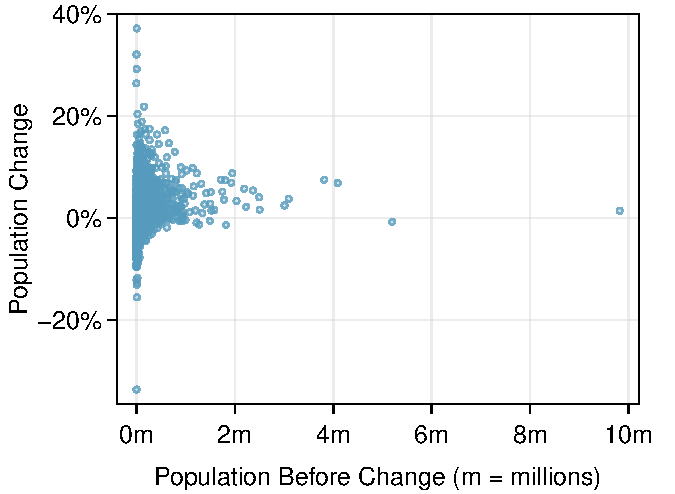
\includegraphics[width=0.47\textwidth]{ch_summarizing_data/figures/county_pop_change_v_pop_transform/county_pop_change_v_pop_transform_i}
\label{county_pop_change_v_pop_transform_i}
}
\subfigure[]{
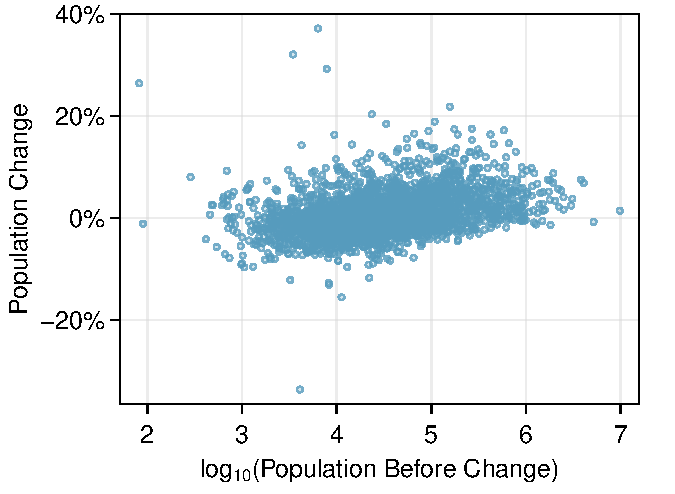
\includegraphics[width=0.47\textwidth]{ch_summarizing_data/figures/county_pop_change_v_pop_transform/county_pop_change_v_pop_transform_log}
\label{county_pop_change_v_pop_transform_log}
}
\caption{\subref{county_pop_change_v_pop_transform_i} Scatterplot of \var{line\_\hspace{0.3mm}breaks} against \var{num\_\hspace{0.3mm}char} for 50 emails. \subref{county_pop_change_v_pop_transform_log} A scatterplot of the same data but where each variable has been log-transformed.}
\label{county_pop_change_v_pop_transform_main}
\end{figure}

Transformations other than the logarithm can be useful, too.
For instance, the square root
($\sqrt{\text{original observation}}$) and inverse
($\frac{1}{\text{original observation}}$) are commonly used
by data scientists.
Common goals in transforming data are to see the data
structure differently, reduce skew, assist in modeling,
or straighten a nonlinear relationship in a scatterplot.

\index{data!county|)}


\subsection{Mapping data (special topic)}

\index{data!county|(}
\index{intensity map|(}

The \data{county} data set offers many numerical variables
that we could plot using dot plots, scatterplots,
or box plots, but these miss the true nature of the data.
Rather, when we encounter geographic data, we should map
it using an \term{intensity map}, where colors are used
to show higher and lower values of a variable.
Figures~\ref{countyIntensityMaps1}
and~\ref{countyIntensityMaps2} shows intensity maps for
poverty rate in percent (\var{poverty}),
unemployment rate (\var{unemployment\_\hspace{0.3mm}rate}),
homeownership rate in percent (\var{homeownership}),
and median household income
(\var{median\_\hspace{0.3mm}hh\_\hspace{0.3mm}income}).
The color key indicates which colors correspond to which values.
The intensity maps are not generally very helpful
for getting precise values in any given county,
but they are very helpful for seeing geographic trends
and generating interesting research questions or hypotheses.

\begin{figure}
\centering
\subfigure[]{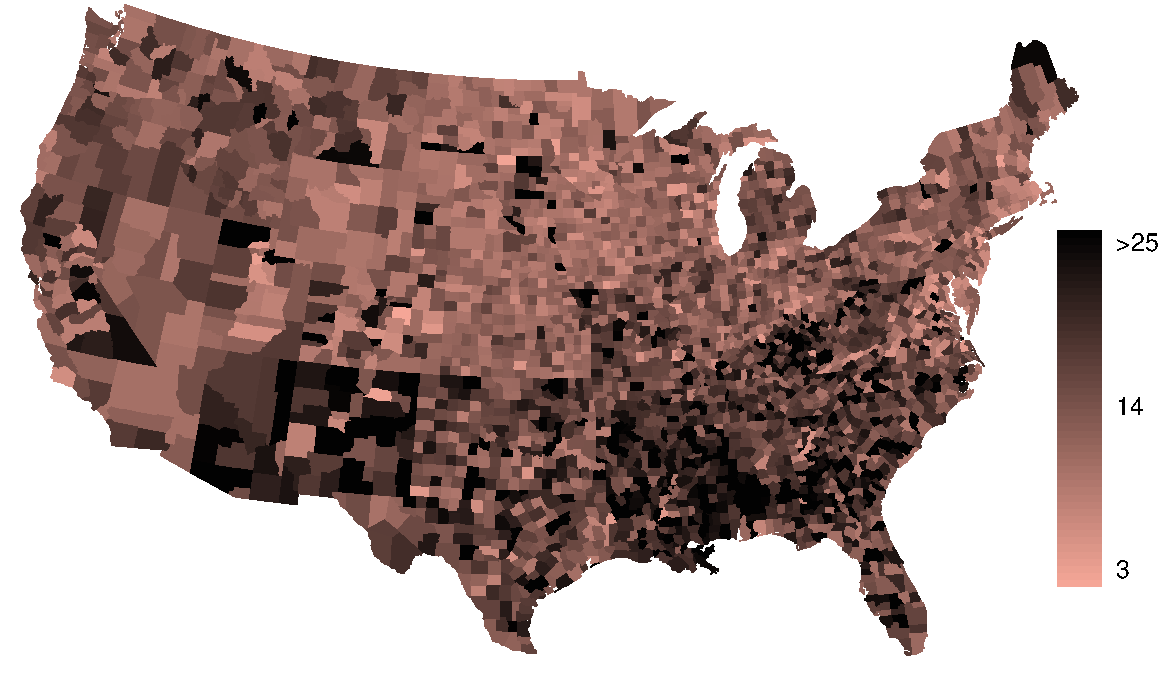
\includegraphics[width=\textwidth]{ch_summarizing_data/figures/countyIntensityMaps/countyPovertyMap}\label{countyPovertyMap}}
\subfigure[]{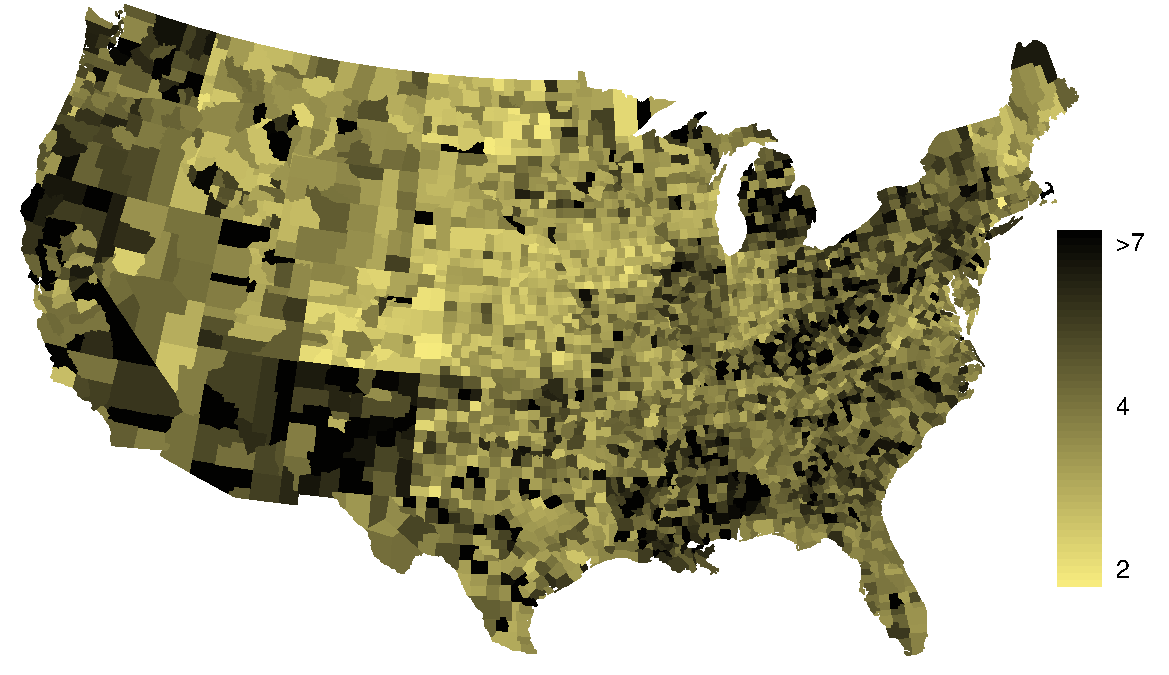
\includegraphics[width=\textwidth]{ch_summarizing_data/figures/countyIntensityMaps/countyUnemploymentRateMap}\label{countyUnemploymentRateMap}}
\caption{\subref{countyPovertyMap} Intensity map of poverty rate (percent). \subref{countyUnemploymentRateMap} Map of the unemployment rate (percent).}
\label{countyIntensityMaps1}
\end{figure}

\begin{figure}
\centering
\subfigure[]{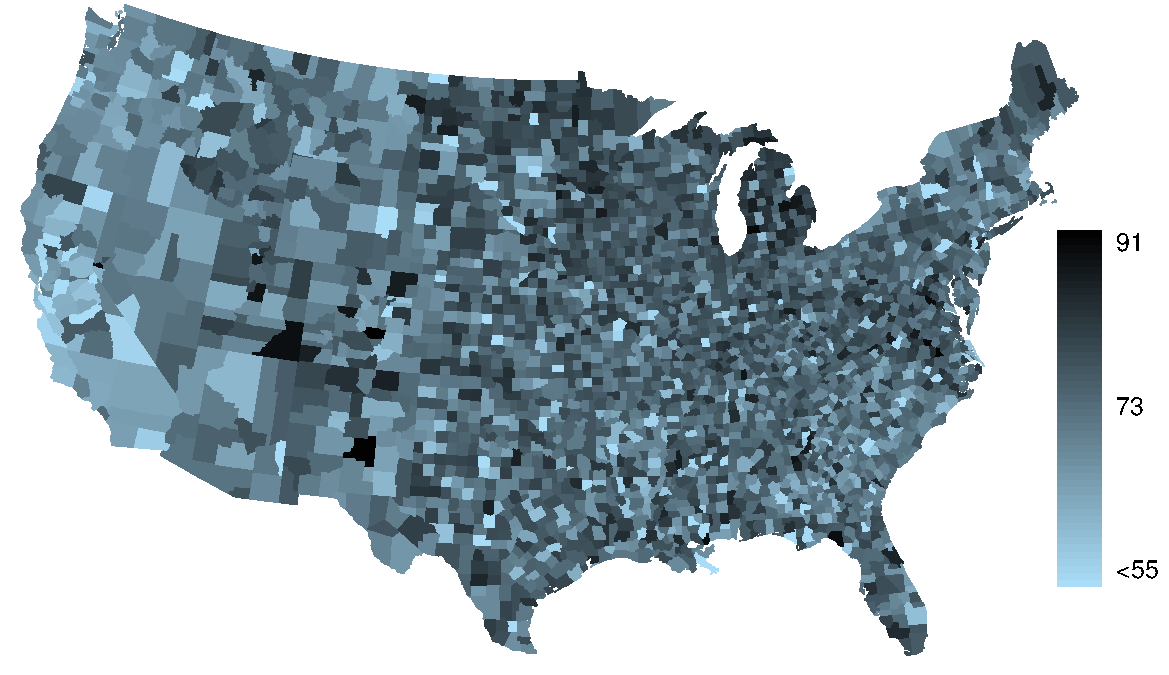
\includegraphics[width=\textwidth]{ch_summarizing_data/figures/countyIntensityMaps/countyHomeownershipMap}\label{countyHomeownershipMap}}
\subfigure[]{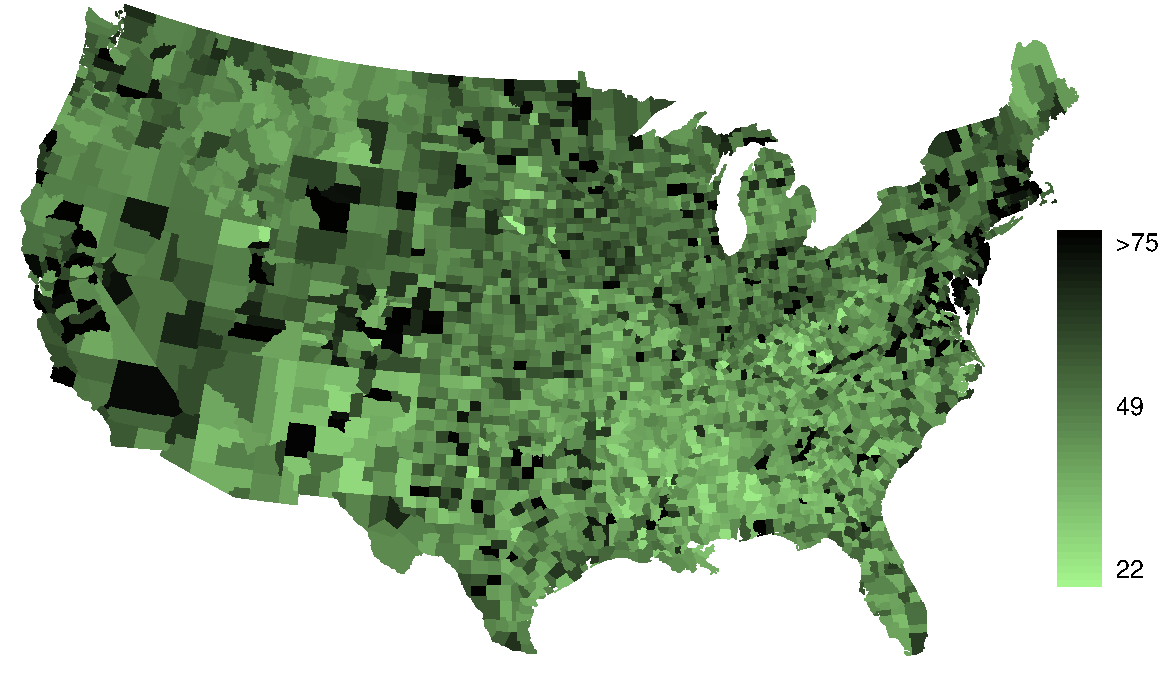
\includegraphics[width=\textwidth]{ch_summarizing_data/figures/countyIntensityMaps/countyMedIncomeMap}\label{countyMedIncomeMap}}
\caption{\subref{countyHomeownershipMap} Intensity map of homeownership rate (percent). \subref{countyMedIncomeMap} Intensity map of median household income (\$1000s).}
\label{countyIntensityMaps2}
\end{figure}

\begin{example}{What interesting features are evident in the
    \var{poverty} and \var{unemployment\_\hspace{0.3mm}rate}
    intensity maps?}
  Poverty rates are evidently higher in a few locations.
  Notably, the deep south shows higher poverty rates,
  as does the southwest border of Texas.
  The vertical strip of eastern Utah and Arizona
  appears to have higher rates of poverty.
  High poverty rates are evident in the Mississippi
  flood plains a little north of New Orleans and
  also in a large section of Kentucky and West Virginia.

  The unemployment rate follows similar trends,
  and we can see correspondence between the two
  variables. In fact, it makes sense for higher rates
  of unemployment to be closely related to poverty rates.
  One observation that stand out when comparing the two maps:
  the poverty rate is much higher than the unemployment
  rate, meaning while many people may be working,
  they are not making enough to break out of poverty.
\end{example}

\begin{exercise}
What interesting features are evident in the \var{median\_\hspace{0.3mm}hh\_\hspace{0.3mm}income} intensity map in Figure~\ref{countyMedIncomeMap}?\footnote{Note: answers will vary. There is a very strong correspondence between high earning and metropolitan areas. You might look for large cities you are familiar with and try to spot them on the map as dark spots.}
\end{exercise}

\index{intensity map|)}
\index{data!county|)}



\section[Considering categorical data]{Considering categorical data \sectionvideohref{youtube-7NhNeADL8fA&list=PLkIselvEzpM6pZ76FD3NoCvvgkj_p-dE8}~\sectionslideshref{gdoc_os3_slides_1-7}}
\label{categoricalData}

\index{data!loans|(}

Like numerical data, categorical data can also be organized
and analyzed.
In this section, we will introduce tables and other basic tools
for categorical data that are used throughout this book.
The \data{loan50} data set represents a sample from a larger
email data set called \data{loans}.
This larger data set contains information on 10,000 loans made
through Lending Club.
In this section we will examine the relationship between
\var{homeownership}, which for the \data{loans} data can take
a value of \resp{rent}, \resp{mortgage}
(owns but has a mortgage), or \resp{own},
and \var{app\_\hspace{0.3mm}type},
which indicates whether the borrower reported joint income
with a partner or whether that reported income was
individual only.
% library(openintro); dim(loans_full_schema)


\subsection{Contingency tables and bar plots}

\newcommand{\loanapphomeAA}{3496}
\newcommand{\loanapphomeAB}{3839}
\newcommand{\loanapphomeAC}{1170}
\newcommand{\loanapphomeAD}{8505}
\newcommand{\loanapphomeBA}{362}
\newcommand{\loanapphomeBB}{950}
\newcommand{\loanapphomeBC}{183}
\newcommand{\loanapphomeBD}{1495}
\newcommand{\loanapphomeDA}{3858}
\newcommand{\loanapphomeDAPt}{0.3858} % Overall frequency
\newcommand{\loanapphomeDB}{4789}
\newcommand{\loanapphomeDC}{1353}
\newcommand{\loanapphomeDD}{10000}
\newcommand{\loanapphomeN}{\loanapphomeDD{}}

Figure~\ref{loan_home_app_type_totals} summarizes two variables:
\var{app\_\hspace{0.3mm}type} and \var{homeownership}.
A table that summarizes data for two categorical variables in
this way is called a \term{contingency table}.
Each value in the table represents the number of times
a particular combination of variable outcomes occurred.
For example, the value \loanapphomeAA{} corresponds to the number of
loans in the data set where the borrower rents their home
and the application type was by an individual.
Row and column totals are also included.
The \term{row totals} \index{contingency table!row totals}
provide the total counts across each row
(e.g. $\loanapphomeAA{} + \loanapphomeAB{} +
  \loanapphomeAC{} = \loanapphomeAD{}$),
and \term{column totals} \index{contingency table!column totals}
are total counts down each column.

A table for a single variable is called a \term{frequency table}.
Figure~\ref{loan_homeownership_totals} is a frequency table for
the \var{homeownership} variable.
If we replaced the counts with percentages or proportions,
the table would be called a \term{relative frequency table}.

\begin{figure}[ht]
\centering
\begin{tabular}{ll  ccc  rr}
& & \multicolumn{3}{c}{\bf \var{homeownership}} & \\
  \cline{3-5}
& & rent & mortgage & own & Total & \hspace{2mm}\  \\ 
  \cline{2-6}
& individual & \loanapphomeAA{} & \loanapphomeAB{} &
      \loanapphomeAC{} & \loanapphomeAD{} \\ 
  
\raisebox{1.5ex}[0pt]{\var{app\_\hspace{0.3mm}type}}
& joint & \loanapphomeBA{} & \loanapphomeBB{} &
	    \loanapphomeBC{} & \loanapphomeBD{} \\ 
  \cline{2-6}
& Total & \loanapphomeDA{} & \loanapphomeDB{} &
    \loanapphomeDC{} & \loanapphomeDD{} \\
  \cline{2-6}
\end{tabular}
\caption{A contingency table for \var{app\_\hspace{0.3mm}type} and \var{homeownership}.}
\label{loan_home_app_type_totals}
%library(openintro); library(xtable); tab <- table(loans_full_schema[,c("application_type", "homeownership")])[, c("RENT", "MORTGAGE", "OWN")]; xtable(tab); rowSums(tab); colSums(tab); sum(tab)
\end{figure}

\begin{figure}[htb]
\centering
\begin{tabular}{lc}
  \hline
\var{homeownership} & Count \\
   \hline
rent & \loanapphomeDA{} \\
mortgage & \loanapphomeDB{} \\
own & \loanapphomeDC{} \\
\hline
Total & \loanapphomeDD{} \\ 
   \hline
\end{tabular}
\caption{A frequency table for the \var{homeownership} variable.}
\label{loan_homeownership_totals}
\end{figure}
%library(openintro); library(xtable); data(email); xtable(table(email[,c("html")]))

A bar plot is a common way to display a single
categorical variable.
The left panel of Figure~\ref{loan_homeownership_bar_plot}
shows a \term{bar plot} for the \var{homeownership} variable.
In the right panel, the counts are converted into proportions
(e.g. $\loanapphomeDA{} / \loanapphomeDD{} = 0.3858$ for
  \resp{rent}),
showing the proportion of observations that are in each level
(i.e. in each category).

\begin{figure}[bht]
   \centering
   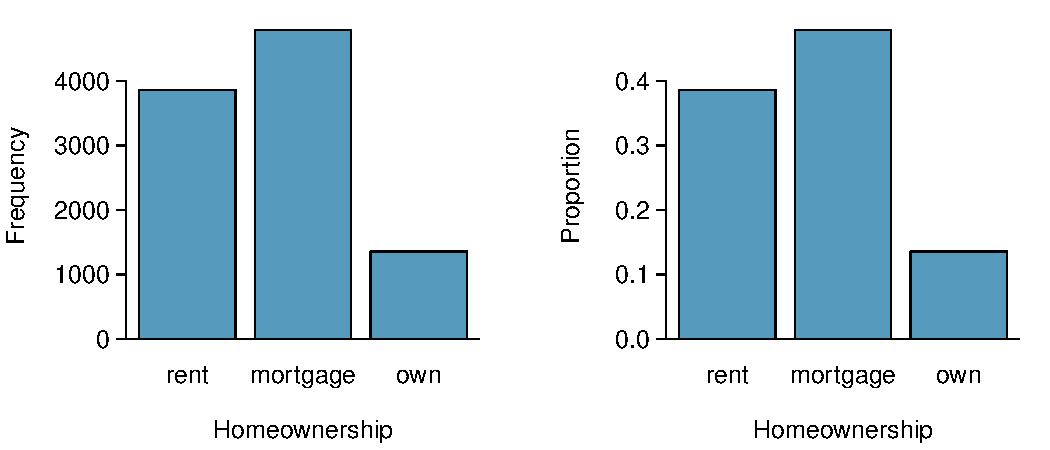
\includegraphics[width=0.9\textwidth]{ch_summarizing_data/figures/loan_homeownership_bar_plot/loan_homeownership_bar_plot}
   \caption{Two bar plots of \var{number}. The left panel shows the counts, and the right panel shows the proportions in each group.}
   \label{loan_homeownership_bar_plot}
\end{figure}


\subsection{Row and column proportions}

Figure~\ref{rowPropAppTypeHomeownership} shows the row proportions for Figure~\ref{loan_home_app_type_totals}. The \termsub{row proportions}{contingency table!row proportions} are computed as the counts divided by their row totals. The value \loanapphomeAA{} at the intersection of \resp{individual} and \resp{rent} is replaced by $\loanapphomeAA{}/\loanapphomeAD{}=0.411$, i.e. \loanapphomeAA{} divided by its row total, \loanapphomeAD{}. So what does 0.411 represent? It corresponds to the proportion of individual applicants who rent.

\begin{figure}
\centering
\begin{tabular}{l rrr r}
  \hline
 & rent & mortgage & own & Total \\
  \hline
individual & 
    $\loanapphomeAA{}/\loanapphomeAD{} = 0.411$ &
    $\loanapphomeAB{}/\loanapphomeAD{} = 0.451$ &
    $\loanapphomeAC{}/\loanapphomeAD{} = 0.138$ &
    1.000 \\
joint &
    $\loanapphomeBA{}/\loanapphomeBD{} = 0.242$ &
    $\loanapphomeBB{}/\loanapphomeBD{} = 0.635$ &
    $\loanapphomeBC{}/\loanapphomeBD{} = 0.122$ &
    1.000 \\
   \hline
Total &
    $\loanapphomeDA{}/\loanapphomeDD{} = 0.386$ &
    $\loanapphomeDB{}/\loanapphomeDD{} = 0.479$ &
    $\loanapphomeDC{}/\loanapphomeDD{} = 0.135$ &
    1.000 \\
  \hline
\end{tabular}
\caption{A contingency table with row proportions for the
  \var{app\_\hspace{0.3mm}type} and \var{homeownership} variables.
  The totals for some rows are off by 0.001 due to rounding errors.}
\label{rowPropAppTypeHomeownership}
\end{figure}

A contingency table of the column proportions is computed in a similar way, where each \termsub{column proportion}{contingency table!column proportion} is computed as the count divided by the corresponding column total. Figure~\ref{colPropAppTypeHomeownership} shows such a table, and here the value 0.906 indicates that 90.6\% of renters applied as individuals for the loan. This rate is higher compared to loans from people with mortgages (80.2\%) or who own their home (85.1\%). Because these rates vary between the three levels of \var{homeownership} (\resp{rent}, \resp{mortgage}, \resp{own}), this provides evidence that the \var{app\_\hspace{0.3mm}type} and \var{homeownership} variables are associated.

\begin{figure}[h]
\centering\small
\begin{tabular}{l rrr r}
  \hline
 & rent & mortgage & own & Total \\
  \hline
individual &
    $\loanapphomeAA{}/\loanapphomeDA{} = 0.906$ &
    $\loanapphomeAB{}/\loanapphomeDB{} = 0.802$ &
    $\loanapphomeAC{}/\loanapphomeDC{} = 0.865$ &
    $\loanapphomeAD{}/\loanapphomeDD{} = 0.851$ \\
joint &
    $\loanapphomeBA{}/\loanapphomeDA{} = 0.094$ &
    $\loanapphomeBB{}/\loanapphomeDB{} = 0.198$ &
    $\loanapphomeBC{}/\loanapphomeDC{} = 0.135$ &
    $\loanapphomeBD{}/\loanapphomeDD{} = 0.150$ \\
   \hline
Total & 1.000 & 1.000 & 1.000 & 1.000 \\
   \hline
\end{tabular}
\caption{A contingency table with column proportions for the
  \var{app\_\hspace{0.3mm}type} and \var{homeownership} variables.
  The total for the last column is off by 0.001 due
  to a rounding error.}
\label{colPropAppTypeHomeownership}
\end{figure}

We could also have checked for an association between \var{app\_\hspace{0.3mm}type} and \var{homeownership} in Figure~\ref{rowPropAppTypeHomeownership} using row proportions. When comparing these row proportions, we would look down columns to see if the fraction of loans where the borrower rents, has a mortgage, or owns varied across the \resp{individual} to \resp{joint} application types.

\Comment{These next exercises must be checked \textbf{very} carefully.}

\begin{exercise}
What does 0.451 represent in Figure~\ref{rowPropAppTypeHomeownership}? What does 0.802 represent in Figure~\ref{colPropAppTypeHomeownership}?\footnote{0.451 represents the proportion of individual applicants who have a mortgage. 0.802 represents the fraction of applicants with mortgages who applied as individuals.}
\end{exercise}

\begin{exercise}
What does 0.122 at the intersection of \resp{joint} and \resp{own} represent in Figure~\ref{rowPropAppTypeHomeownership}? What does 0.135 represent in the Figure~\ref{colPropAppTypeHomeownership}?\footnote{0.122 represents the fraction of joint borrowers who own their home. 0.135 represents the home-owning borrowers who had a joint application for the loan.}
\end{exercise}

\begin{example}{
%To evaluate the riskiness of a loan, brokers take into account many variables. However, sometimes those pieces of information are very closely associated, meaning their information is somewhat redundant. Do the 
Data scientists use statistics to filter spam from incoming
email messages.
By noting specific characteristics of an email,
a data scientist may be able to classify some emails as spam
or not spam with high accuracy.
One of those characteristics is whether the email
contains no numbers, small numbers, or big numbers.
Another characteristic is whether or not an email
has any HTML content.
A contingency table for the \var{spam} and \var{format}
variables from the \data{email} data set are shown in
Figure~\ref{emailSpamHTMLTableTotals}.
For reference, an HTML email is an email with the capacity
for special formatting, e.g. bold text.
In Figure~\ref{emailSpamHTMLTableTotals},
which would be more helpful to someone hoping to classify
email as spam or regular email: row or column proportions?} \label{weighingRowColumnProportions}
A data scientist would be interested in how the proportion
of spam changes within each email format.
This corresponds to column proportions:
the proportion of spam in plain text emails
and the proportion of spam in HTML emails.

If we generate the column proportions, we can see
that a higher fraction of plain text emails are
spam ($209/1195 = 17.5\%$)
than compared to HTML emails ($158/2726 = 5.8\%$).
This information on its own is insufficient to classify
an email as spam or not spam, as over 80\% of plain text
emails are not spam.
Yet, when we carefully combine this information with many
other characteristics, such as \var{number} and other variables,
we stand a reasonable chance of being able to classify some
email as spam or not spam.
%\GLMSection{This is a topic we will return to in
%Chapter~\ref{multipleRegressionAndANOVA}.}{}
\end{example}

\begin{figure}[ht]
\centering
\begin{tabular}{l cc r}
  \hline
 & text & HTML & Total \\ 
  \hline
spam & 209 & 158 & 367 \\ 
not spam & 986 & 2568 & 3554 \\ 
   \hline
Total & 1195 & 2726 & 3921 \\
   \hline
\end{tabular}
\caption{A contingency table for \var{spam} and \var{format}.}
\label{emailSpamHTMLTableTotals}
%library(openintro); library(xtable); data(email); tab <- table(email[,c("spam", "format")])[2:1,]; tab; colSums(tab); rowSums(tab)
\end{figure}

\Comment{This next discussion and following example
  are relatively new.}
Example~\ref{weighingRowColumnProportions} points out
that row and column proportions are not equivalent.
Before settling on one form for a table,
it is important to consider each to ensure that the
most useful table is constructed.
However, sometimes it simply isn't clear which, if either,
is more useful.

\begin{example}{Look back to
    Tables~\ref{rowPropAppTypeHomeownership}
    and~\ref{colPropAppTypeHomeownership}.
    Are there any obvious scenarios where one might be more
    useful than the other?}
  None that we thought were obvious!
  What is distinct about \var{app\_\hspace{0.3mm}type}
  and \var{homeownership} vs the email example is that
  these two variables don't have a clear explanatory-response
  variable relationship that we might hypothesize
  (these terms were introduced in
    Section~\ref{explanatoryAndResponse}).
  Usually it is most useful to ``condition'' on the
  explanatory variable.
  For instance, in the email example, the email format
  was seen as a possible explanatory variable of whether
  the message was spam, so we computed the relative
  frequencies for each email format.
\end{example}

\Comment{Any risk with the above example that students
  would think they need not know how to describe (what
  are effectively) conditional probabilities based
  on row or column proportions?
  If so, we could add in an exercise that calls this
  out and requires them to create such a description.}


\subsection{Using a bar plot with two variables}
\label{bar_plots_subsection}

Contingency tables using row or column proportions
are especially useful for examining how two categorical
variables are related.
Stacked bar plots provide a way to visualize
the information in these tables.

A \termsub{stacked bar plot}{bar plot!stacked bar plot}
\index{bar plot!segmented bar plot}
is a graphical display of contingency table information.
For example, a stacked bar plot representing
Figure~\ref{colPropAppTypeHomeownership}
is shown in Figure~\ref{loan_app_type_home_seg_bar},
where we have first created a bar plot using the
\var{homeownership} variable and then divided each group
by the levels of \var{app\_\hspace{0.3mm}type}.
One related visualization is a
\termsub{side-by-side bar plot}{bar plot!side-by-side},
which is shown in
Figure~\ref{loan_app_type_home_sbs_bar}.
The column proportions of
Figure~\ref{colPropAppTypeHomeownership}
have been translated into a standardized stacked bar plot
in Figure~\ref{loan_app_type_home_seg_bar_standardized},
which is a helpful visualization of the fraction of individual
or joint loan applications for borrowers in each level of
\var{homeownership}.


\newcommand{\loanapptypehomesegbarplotwidth}{0.48\textwidth}
\begin{figure}[h]
\centering
\subfigure[]{
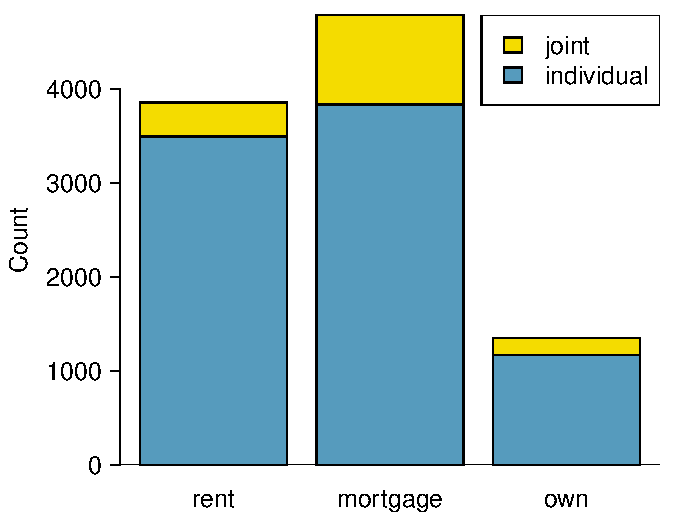
\includegraphics[width=\loanapptypehomesegbarplotwidth]{ch_summarizing_data/figures/loan_app_type_home_seg_bar/loan_app_type_home_seg_bar}
\label{loan_app_type_home_seg_bar}
}
\subfigure[]{
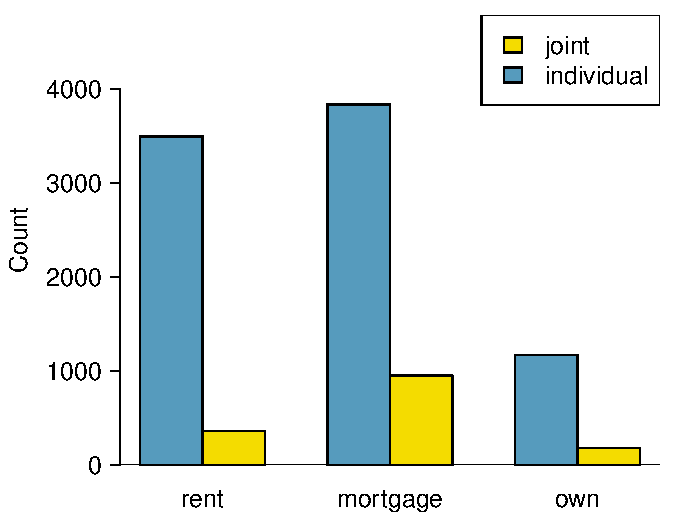
\includegraphics[width=\loanapptypehomesegbarplotwidth]{ch_summarizing_data/figures/loan_app_type_home_seg_bar/loan_app_type_home_sbs_bar}
\label{loan_app_type_home_sbs_bar}
}
\subfigure[]{
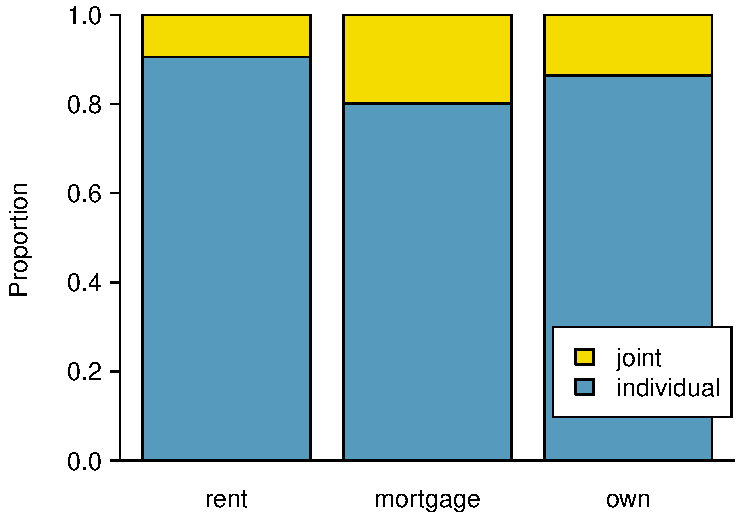
\includegraphics[width=\loanapptypehomesegbarplotwidth]{ch_summarizing_data/figures/loan_app_type_home_seg_bar/loan_app_type_home_seg_bar_standardized}
\label{loan_app_type_home_seg_bar_standardized}
}
\caption{\subref{loan_app_type_home_seg_bar} Stacked
  bar plot for \var{homeownership},
  where the counts have been further broken down
  by \var{app\_\hspace{0.3mm}type}.
  \subref{loan_app_type_home_sbs_bar}~Side-by-side
  bar plot for \var{homeownership}
  and \var{app\_\hspace{0.3mm}type}.
  \subref{loan_app_type_home_seg_bar_standardized}~Standardized
  version of the stacked bar plot.}
\label{loan_app_type_home_seg_bar_plot}
\end{figure}

\begin{example}{Examine the three bar plots in
    Figure~\ref{loan_app_type_home_seg_bar_plot}.
    When is the stacked, side-by-side, or standardized
    stacked bar plot the most useful?}
  This stacked bar plot is most useful when it is reasonable
  to assign one variable as the explanatory variable and
  the other variable as the response, since we are effectively
  grouping by one variable first and then breaking it down by
  the others.

  Side-by-side bar plots are more agnostic in their display
  about which variable, if any, represents the explanatory
  and which the response variable.
  It is also easy to discern the number of cases
  in of the six different group combinations shown than
  in a stacked bar plot.
  However, one downside of the side-by-side visualization
  is that it tends to require more horizontal space;
  the narrowness of Figure~\ref{loan_app_type_home_sbs_bar}
  makes the plot feel a bit cramped.
  Additionally, when two groups are of very different sizes,
  as we see in the \resp{mortgage} and \resp{own} groups,
  it is difficult to discern if there is any association
  between the variables.

  The standardized stacked bar plot is helpful if primary
  variable in the stacked bar plot is relatively imbalanced,
  e.g. as we see where the \resp{own} category has only
  a third of the observations in the \resp{mortgage}
  category, making it a bit more difficult
  to discern whether the proportion of borrowers
  in each group that are individual or joint borrowers
  is stable across the two groups.
  That said, the major downside of the standardized version
  is that we lose all sense of how many cases each of the
  bars represents.
\end{example}

%Before settling on a particular bar plot, consider each
%carefully.
%It can also be useful to make a couple of the versions,
%which will offer different views and insights into the data
%than if only one bar plot variant is reviewed.

\subsection{Mosaic plots}
\label{mosaic_plots_subsection}

A \term{mosaic plot} is a visualization technique
suitable for contingency tables that resembles
a standardized stacked bar plot with the benefit
that we still see the relative group sizes of the
primary variable.

To get started in creating our first mosaic plot,
we'll break a square into columns for each category
of the \var{homeownership} variable,
with the result shown in Figure~\ref{loan_home_mosaic}.
Each column represents a level of \var{homeownership},
and the column widths correspond to the proportion of
loans in each of those categories.
For~instance, there are fewer loans where the borrower
is an owner than where the borrower has a mortgage.
In general, mosaic plots use box \emph{areas}
to represent the number of cases in each category.

\begin{figure}[h]
\centering
\subfigure[]{
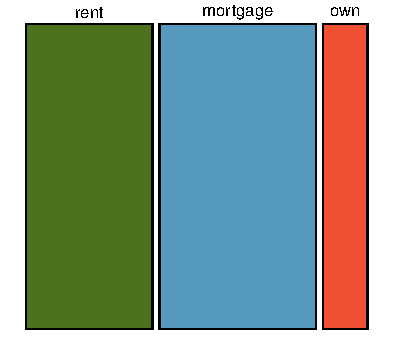
\includegraphics[width=0.36\textwidth]{ch_summarizing_data/figures/loan_app_type_home_mosaic_plot/loan_home_mosaic}
\label{loan_home_mosaic}
}
\subfigure[]{
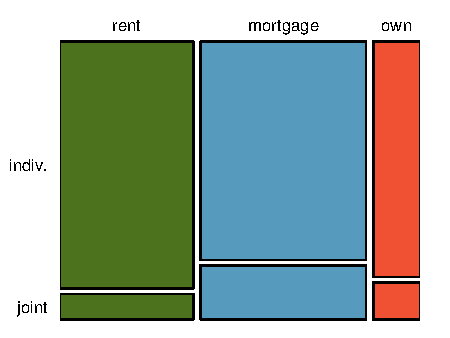
\includegraphics[width=0.44\textwidth]{ch_summarizing_data/figures/loan_app_type_home_mosaic_plot/loan_app_type_home_mosaic}
\label{loan_app_type_home_mosaic}
}
\caption{\subref{loan_home_mosaic}~The one-variable mosaic
    plot for \var{homeownership}.
    \subref{loan_app_type_home_mosaic}~Two-variable mosaic
    plot for both \var{homeownership}
    and \var{app\_\hspace{0.3mm}type}.}
\label{loan_app_type_home_mosaic_plot}
\end{figure}

To create a completed mosaic plot, the single-variable
mosaic plot is further divided into pieces in
Figure~\ref{loan_app_type_home_mosaic} using the
\var{app\_\hspace{0.3mm}type} variable.
Each column is split proportional to the
number of loans from individual and joint
borrowers.
For example, the second column represents loans
where the borrower has a mortgage,
and it was divided into individual loans (upper)
and joint loans (lower).
As another example, the bottom segment of the third column
represents loans where the borrower owns their home
and applied jointly, while the upper segment represents
borrowers who are homeowners and filed individually.
We can again use this plot to see that
the \var{homeownership} and \var{app\_\hspace{0.3mm}type}
variables are associated, since some columns are divided
in different vertical locations than others,
which was the same technique used for checking an
association in the standardized stacked bar plot.

In Figure~\ref{loan_app_type_home_mosaic_rev},
we chose to first split by the homeowner status
of the borrower.
However, we could have instead first split by
the application type, as in
Figure~\ref{loan_app_type_home_mosaic_rev}.
Like with the bar plots, it's common to use
the explanatory variable to represent the
first split in a mosaic plot,
and then for the response to break
up each level of the explanatory variable.

\begin{figure}[h]
   \centering
   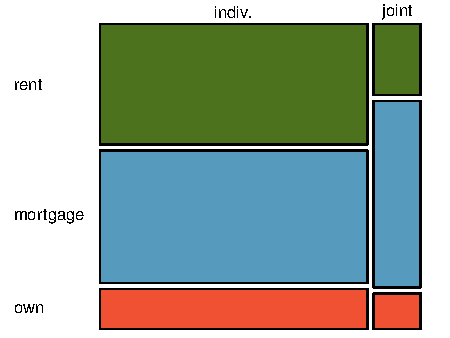
\includegraphics[width=0.37\textwidth]{ch_summarizing_data/figures/loan_app_type_home_mosaic_plot/loan_app_type_home_mosaic_rev}
   \caption{Mosaic plot where emails are grouped by the \var{homeownership} variable after they've been divided into the \resp{individual} and \resp{joint} application types.}
   \label{loan_app_type_home_mosaic_rev}
\end{figure}

%In a similar way, a mosaic plot representing row proportions of Figure~\ref{loan_home_app_type_totals} could be constructed, as shown in Figure~\ref{loan_app_type_home_mosaic_rev}. However, because it is more insightful for this application to consider the fraction of spam in each category of the \var{number} variable, we prefer Figure~\ref{loan_app_type_home_mosaic}.


\subsection{The only pie chart you will see in this book}

\Comment{Softening the language against pie charts.}

A \term{pie chart} is shown in
Figure~\ref{loan_homeownership_pie_chart} alongside
a bar plot representing the same information.
Pie charts can be useful for giving a high-level overview
to show how a set of cases break down.
However, it is also difficult to decipher close details
in a pie chart.
For example, it takes a little longer to recognize
that there are more loans where the borrower has
a mortgage than rent when looking at the pie chart,
while this detail is very obvious in the bar plot.
%One benefit of pie charts is that they to make it easier
%to see when a series of groups make up at least 50\%,
%e.g. \Comment{would need to show a pie chart with
%  a large number of categories for this point to make sense}.

\begin{figure}[h]
   \centering
   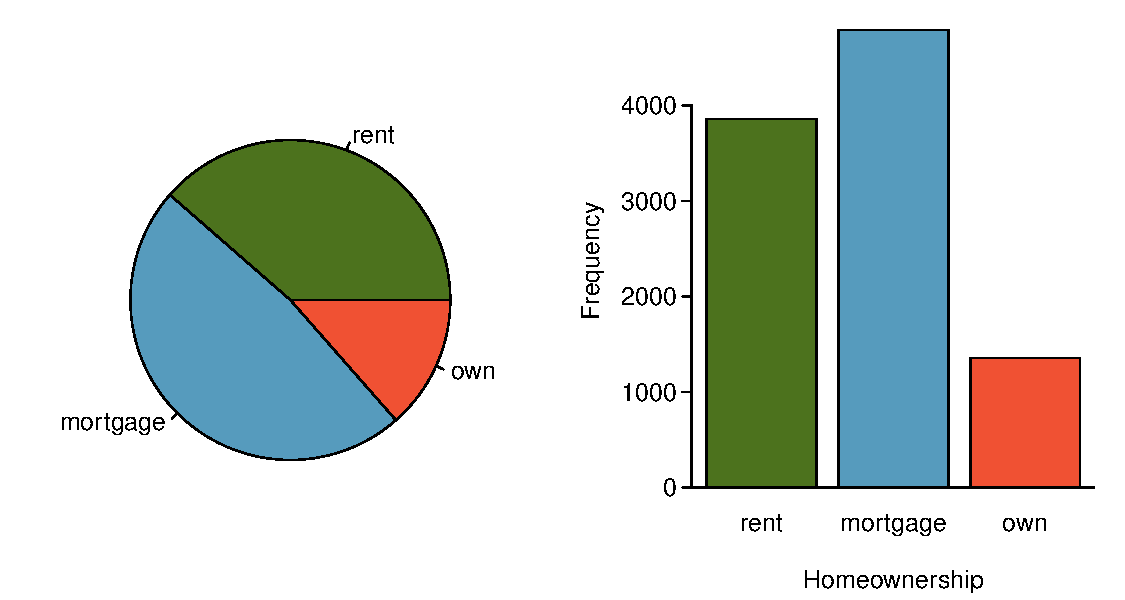
\includegraphics[width=\textwidth]{ch_summarizing_data/figures/loan_homeownership_pie_chart/loan_homeownership_pie_chart}
   \caption{A pie chart and bar plot of \var{homeownership}.}
   \label{loan_homeownership_pie_chart}
\end{figure}

\index{data!loans|)}

\subsection{Comparing numerical data across groups}
\label{comparingAcrossGroups}

\index{data!county|(}

Some of the more interesting investigations can be considered
by examining numerical data across groups.
The methods required here aren't really new.
All that is required is to make a numerical plot for each group.
Here two convenient methods are introduced: side-by-side
box plots and hollow histograms.

We will take a look again at the \data{county} data set
and compare the median household income for counties that
gained population from 2010 to 2017 versus counties that
had no gain.\footnote{Some counties are excluded since
  they did not have available population data for one
  or both years.}
While we might like to make a causal connection here,
remember that these are observational data and so such
an interpretation would not be justified.

\newcommand{\numcountieswithgains}{1454}
\newcommand{\numcountieswithgainsC}{1,454}
\newcommand{\numcountieswithoutgains}{1672}
\newcommand{\numcountieswithoutgainsC}{1,672}

There were \numcountieswithgainsC{} counties where
the population increased from 2010 to 2017, and there
were \numcountieswithoutgainsC{} counties with no gain
(all but one were a loss).
A~random sample of 100 counties from the first group and
50 from the second group are shown in
Figure~\ref{countyIncomeSplitByPopGainTable}
to give a better sense of some of the raw median
income data.

\begin{figure}
\centering
\begin{tabular}{ ccc ccc c ccc }
\multicolumn{6}{c}{\bf population gain} &&
    \multicolumn{3}{c}{\bf no gain} \\ 
  \cline{1-6} \cline{8-10}
62.7 & 61.2 & 32.4 & 74.2 & 44.6 & 38.8 &\hspace{5mm}\ &
    55.2 & 49.6 & 44.1 \\
26.7 & 63.6 & 42.9 & 45.3 & 52.8 & 77 && 41.1 & 45.8 & 49 \\
41.5 & 45.3 & 55.5 & 49 & 38.2 & 51 && 53.9 & 44.8 & 38.8 \\
48.1 & 45.6 & 74.1 & 50.6 & 45.6 & 97.5 && 54.6 & 41.5 & 44.1 \\
73.3 & 52.6 & 73.7 & 42.4 & 77.9 & 43.5 && 45.2 & 53.9 & 45.8 \\
74.3 & 49.4 & 55.9 & 57.5 & 36.7 & 54.3 && 36.4 & 49.6 & 47.1 \\
38.9 & 44.9 & 46.6 & 42.1 & 51.8 & 46.2 && 44.8 & 38.7 & 34.5 \\
70.2 & 36.9 & 54.9 & 85.7 & 50.7 & 42 && 56.1 & 53.3 & 37.8 \\
43.2 & 66 & 53 & 40.8 & 48 & 81.6 && 29 & 32.7 & 44.5 \\
58.5 & 45.4 & 47.4 & 94.7 & 65.5 & 54.9 && 39.7 & 26.6 & 38.4 \\
76.8 & 60.8 & 40.5 & 52 & 45.9 & 67.7 && 51.6 & 35 & 44.6 \\
52.3 & 61.1 & 55.9 & 52.2 & 54.3 & 52.7 && 57.2 & 40.6 & 54.7 \\
56.8 & 76 & 53.4 & 71.2 & 54.7 & 56.8 && 48.1 & 55.3 & 40.3 \\
56.2 & 57.9 & 44.5 & 58 & 101.9 & 63.9 && 46.2 & 33 & 56.7 \\
51.1 & 53.4 & 45.7 & 38.6 & 42 & 55.3 && 41.8 & 47.3 & 56.5 \\
57.6 & 59.6 & 44.6 & 59.2 & 54 &  && 37.6 & 42.9 & 38.9 \\
50.2 & 38.4 & 61.3 & 53.8 & 45.1 &  && 44.3 & 56.3 &  \\
\cline{1-6} \cline{8-10}
\end{tabular}
\caption{In this table, median household income (in \$1000s)
    from a random sample of 100 counties that had population
    gains are shown on the left.
    Median incomes from a random sample of 50 counties that
    had no population gain are shown on the right.}
\label{countyIncomeSplitByPopGainTable}
\end{figure}

The \term{side-by-side box plot}
\index{box plot!side-by-side box plot}
is a traditional tool for comparing across groups.
An example is shown in the left panel of
Figure~\ref{countyIncomeSplitByPopGain},
where there are two box plots, one for each group,
placed into one plotting window and drawn on the same scale.

\begin{figure}
   \centering
   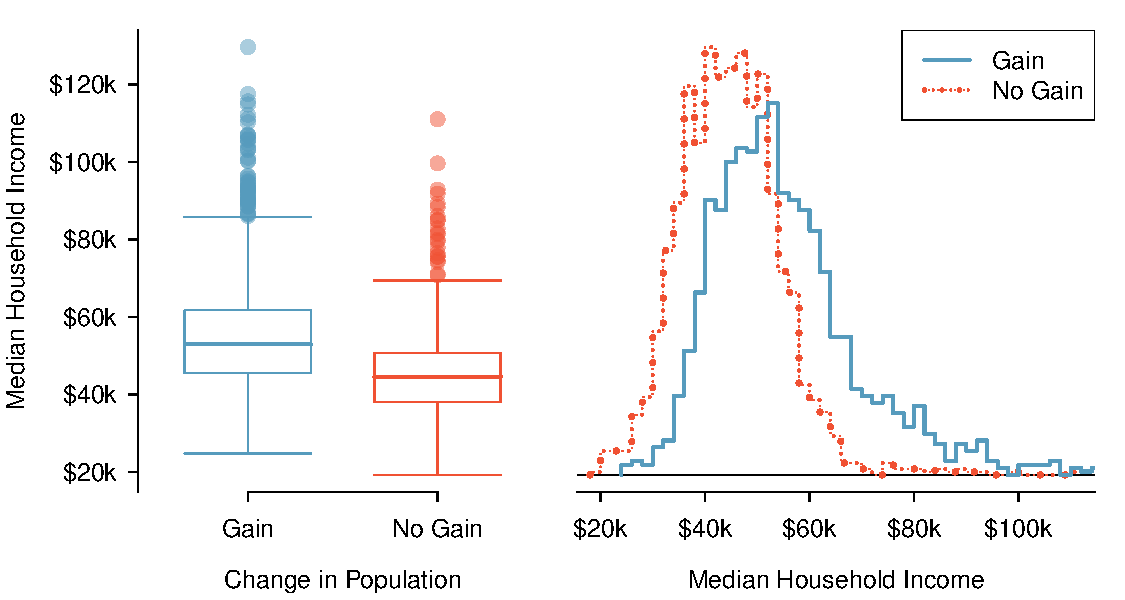
\includegraphics[width=\textwidth]{ch_summarizing_data/figures/countyIncomeSplitByPopGain/countyIncomeSplitByPopGain}
   \caption{Side-by-side box plot (left panel)
       and hollow histograms (right panel) for
       \var{med\_\hspace{0.3mm}hh\_\hspace{0.3mm}income},
       where the counties are split by whether there was
       a population gain or loss.}
   \label{countyIncomeSplitByPopGain}
\end{figure}

Another useful plotting method uses \termsub{hollow histograms}{hollow histogram} to compare numerical data across groups. These are just the outlines of histograms of each group put on the same plot, as shown in the right panel of Figure~\ref{countyIncomeSplitByPopGain}.

\begin{exercise} \label{comparingPriceByTypeExercise}
Use the plots in Figure~\ref{countyIncomeSplitByPopGain}
to compare the incomes for counties across the two groups.
What do you notice about the approximate center of each group?
What do you notice about the variability between groups?
Is the shape relatively consistent between groups?
How many \emph{prominent} modes are there for each
group?\footnote{Answers may vary a little.
  The counties with population gains tend to have higher
  income (median of about \$45,000) versus counties without
  a gain (median of about \$40,000).
  The variability is also slightly larger for the population
  gain group.
  This is evident in the IQR, which is about 50\% bigger
  in the \emph{gain} group.
  Both distributions show slight to moderate right
  skew\index{skew!example: slight to moderate}
  and are unimodal.
  The box plots indicate there are many observations
  far above the median in each group, though we should
  anticipate that many observations will fall beyond
  the whiskers when using such most data sets that
  contain more than a couple hundred data points.}
\end{exercise}

\begin{exercise}
What components of each plot in Figure~\ref{countyIncomeSplitByPopGain} do you find most useful?\footnote{Answers will vary. The side-by-side box plots are especially useful for comparing centers and spreads, while the hollow histograms are more useful for seeing distribution shape, skew, and potential anomalies.}
\end{exercise}

\index{data!county|)}


%___________________________________________
\section[Case study: malaria vaccine (special topic)]
  {Case study: malaria vaccine\\(special topic)}% \sectionvideohref{youtube-2pHhjx9hyM4&list=PLkIselvEzpM6pZ76FD3NoCvvgkj_p-dE8}~\sectionslideshref{gdoc_os3_slides_1-8} \\(special topic)}
\label{caseStudyGenderDiscrimination}

\begin{example}{Suppose your professor splits the students in class into two groups: students on the left and students on the right. If $\hat{p}_{_L}$ and $\hat{p}_{_R}$ represent the proportion of students who own an Apple product on the left and right, respectively, would you be surprised if $\hat{p}_{_L}$ did not {exactly} equal $\hat{p}_{_R}$?}\label{classRightLeftSideApple}
While the proportions would probably be close to each other, it would be unusual for them to be exactly the same. We would probably observe a small difference due to {chance}.
\end{example}

\begin{exercise}
If we don't think the side of the room a person sits on in class is related to whether the person owns an Apple product, what assumption are we making about the relationship between these two variables?\footnote{We would be assuming that these two variables are independent.}
\end{exercise}

\subsection{Variability within data}
\label{variabilityWithinData}

\index{data!malaria vaccine|(}

We consider a study from 2017 on a new malaria vaccine
called PfSPZ.\footnote{Lyke et al. 2017.
  PfSPZ vaccine induces strain-transcending T cells
  and durable protection against heterologous controlled
  human malaria infection.
  PNAS 114(10):2711-2716.}
In this study, volunteer patients were randomized
into one of two experiment groups:
14 patients received an experimental vaccine
or 6 patients received a placebo vaccine.
Nineteen weeks later, all 20 patients were exposed
to a drug-sensitive malaria virus strain;
the motivation of using a drug-sensitive strain
of virus here is for ethical considerations,
allowing any infections to be treated effectively.
The results are summarized in
Figure~\ref{malaria_vaccine_20_exp_summary},
where 9 of the 14 treatment patients remained free
of signs of infection while all of the~6 patients
in the control group patients showed some baseline
signs of infection.

\begin{figure}[ht]
\centering
\begin{tabular}{l l cc rr}
& & \multicolumn{2}{c}{\var{outcome}} \\
  \cline{3-4}
  &  &  {infection} & {no infection} & Total & \hspace{3mm}  \\ 
  \cline{2-5} & {vaccine} & 5 & 9 & 14 \\ 
  \raisebox{1.5ex}[0pt]{\var{treatment}}
      & {placebo} & 6 & 0 & 6 \\ 
  \cline{2-5}
      & Total & 11 & 9 & 20 \\
  \cline{2-5}
\end{tabular}
\caption{Summary results for the malaria vaccine experiment.}
\label{malaria_vaccine_20_exp_summary}
\end{figure}

\begin{exercise}
Is this an observational study or an experiment?
What implications does the study type have on what can
be inferred from the results?\footnote{The
  study is an experiment, as patients were randomly
  assigned an experiment group.
  Since this is an experiment, the results can be used
  to evaluate a causal relationship between the malaria
  vaccine and whether patients showed signs
  of an infection.}
\end{exercise}

In this study, a smaller proportion of patients
who received the vaccine showed signs of an infection
(0.357 versus 1.000).
However, the sample is very small,
and it is unclear whether the difference provides
\emph{convincing evidence} that the vaccine is
effective.

\begin{example}{Data scientists are sometimes called
    upon to evaluate the strength of evidence.
    When looking at the rates of infection for patients
    in the two groups in this study,
    what comes to mind as we try to determine whether
    the data show convincing evidence of a real difference?}
  \label{malaria_vaccine_20_what_is_convincing}
  The observed infection rates
  (35.7\% for the treatment group versus
  100.0\% for the control group)
  suggest the vaccine may be effective.
  However, we cannot be sure if the observed difference
  represents the vaccine's efficacy or is just from
  random chance.
  Generally there is a little bit of fluctuation
  in sample data, and we wouldn't expect the sample
  proportions to be \emph{exactly} equal,
  even if the truth was that the promotion decisions
  were independent of gender.
  Additionally, with such small samples,
  perhaps it's common to observe such large differences
  when we randomly split a group due to chance alone!
\end{example}

Example~\ref{malaria_vaccine_20_what_is_convincing}
is a reminder that the observed outcomes in the data
sample may not perfectly reflect the true relationships
between variables since there is \term{random noise}.
While the observed difference in rates of infection
is large, the sample size for the study is small,
making it unclear if this observed difference represents
efficacy of the vaccine or whether it is simply due to
chance.
We label these two competing claims, $H_0$ and $H_A$:
\begin{itemize}
\setlength{\itemsep}{0mm}
\item[$H_0$:] \textbf{Independence model.}
    The variables \var{treatment} and \var{outcome}
    are independent.
    They have no relationship, and the observed difference
    between the proportion of patients who developed
    an infection in the two groups, 64.3\%, was due to chance.
\item[$H_A$:] \textbf{Alternative model.}
    The variables are \emph{not} independent.
    The difference in infection rates of 64.3\%
    was not due to chance,
    and vaccine affected the rate of infection.
\end{itemize}

What would it mean if the independence model,
which says the vaccine had no influence on the
rate of infection, is true?
It would mean 11~patients were going to develop
develop an infection \emph{no matter which group
they were randomized into},
and 9~patients would not develop an infection
\emph{no matter which group they were randomized
into}.
That~is, if the vaccine did not affect the rate
of infection, the difference in the infection rates
was due to chance alone in how the patients were
randomized.

Now consider the alternative model:
infection rates were influenced by whether a patient
received the vaccine or not.
If this was true, and especially if this influence
was substantial, we would expect to see some difference
in the infection rates of patients in the groups.

We choose between these two competing claims
by assessing if the data conflict so much with
$H_0$ that the independence model cannot be deemed
reasonable.
If this is the case, and the data support $H_A$,
then we will reject the notion of independence
and conclude there was discrimination.


\subsection{Simulating the study}
\label{simulatingTheStudy}

We're going to implement
\termsub{simulations}{simulation},
where we will pretend we know that the malaria
vaccine being tested does \emph{not} work.
Ultimately, we want to understand if the large
difference we observed is common in these
simulations.
If it is common, then maybe the difference
we observed was purely due to chance.
If it is very uncommon, then the possibility
that the vaccine was helpful seems more plausible.

Figure~\ref{malaria_vaccine_20_exp_summary}
shows that 11 patients developed infections and 9 did not.
For our simulation, we will suppose the infections
were independent of the vaccine and we were able to
\emph{rewind} back to when the researchers randomized
the patients in the study.
If we happened to randomize the patients differently,
we may get a different result in this hypothetical
world where the vaccine doesn't influence the infection.
Let's complete another \term{randomization} using
a simulation.

In this \term{simulation}, we take 20 notecards to
represent the 20 patients, where we write down ``infection''
on 11 cards and ``no infection'' on 9 cards.
In this hypothetical world, we believe each patient
that got an infection was going to get it regardless
of which group they were in, so let's see what happens
if we randomly assign the patients to the treatment
and control groups again.
We thoroughly shuffle the notecards and deal 14 into
a \resp{vaccine} pile and 6 into a \resp{placebo} pile.
Finally, we tabulate the results, which are shown in
Figure~\ref{malaria_vaccine_20_exp_summary_rand_1}.

\begin{figure}[ht]
\centering
\begin{tabular}{l l cc rr}
& & \multicolumn{2}{c}{\var{outcome}} \\
  \cline{3-4}
  &  &  {infection} & {no infection} & Total & \hspace{3mm}  \\ 
  \cline{2-5}
   treatment & {vaccine} & 7 & 7 & 14 \\ 
   (simulated) & {placebo} & 4 & 2 & 6 \\ 
  \cline{2-5}
      & Total & 11 & 9 & 20 \\
  \cline{2-5}
\end{tabular}
\caption{Simulation results, where any difference
    in infection rates is purely due to chance.}
\label{malaria_vaccine_20_exp_summary_rand_1}
\end{figure}

\begin{exercise}
\label{malaria_vaccine_20_exp_summary_rand_1_diff}
What is the difference in infection rates between
the two simulated groups in
Figure~\ref{malaria_vaccine_20_exp_summary_rand_1}?
How does this compare to the observed 64.3\% difference
in the actual data?\footnote{$4 / 6 - 7 / 14 = 0.167$
or about 16.7\% in favor of the vaccine.
This difference due to chance is much smaller than the
difference observed in the actual groups.}
\end{exercise}


\subsection{Checking for independence}

We computed one possible difference under the independence model in Guided Practice~\ref{malaria_vaccine_20_exp_summary_rand_1_diff}, which represents one difference due to chance. While in this first simulation, we physically dealt out files, it is more efficient to perform this simulation using a computer. Repeating the simulation on a computer, we get another difference due to chance: -0.042. And another: 0.208. And so on until we repeat the simulation enough times that we have a good idea of what represents the \emph{distribution of differences from chance alone}. Figure~\ref{discRandDotPlot} shows a plot of the differences found from 100 simulations, where each dot represents a simulated difference between the proportions of male and female files that were recommended for promotion.

\begin{figure}[ht]
\centering
\includegraphics[width=0.85\textwidth]{ch_summarizing_data/figures/discRandDotPlot/discRandDotPlot}
\caption{A stacked dot plot of differences from 100 simulations produced under the independence model, $H_0$, where \var{gender\_\hspace{0.3mm}sim} and \var{decision} are independent. Two of the 100 simulations had a difference of at least 29.2\%, the difference observed in the study.}
\label{discRandDotPlot}
\end{figure}

Note that the distribution of these simulated differences is centered around 0. We simulated these differences assuming that the independence model was true, and under this condition, we expect the difference to be zero with some random fluctuation. We would generally be surprised to see a difference of \emph{exactly} 0: sometimes, just by chance, the difference is higher than 0, and other times it is lower than zero.

\begin{example}{How often would you observe a difference of at least 29.2\% (0.292) according to Figure~\ref{discRandDotPlot}? Often, sometimes, rarely, or never?}
It appears that a difference of at least 29.2\% due to chance alone would only happen about 2\% of the time according to Figure~\ref{discRandDotPlot}. Such a low probability indicates a rare event.
\end{example}

The difference of 29.2\% being a rare event suggests two possible interpretations of the results of the study:
\begin{itemize}
\setlength{\itemsep}{0mm}
\item[$H_0$] \textbf{Independence model.} Gender has no effect on promotion decision, and we observed a difference that would only happen rarely.
\item[$H_A$] \textbf{Alternative model.} Gender has an effect on promotion decision, and what we observed was actually due to equally qualified women being discriminated against in promotion decisions, which explains the large difference of 29.2\%.
\end{itemize}
Based on the simulations, we have two options. (1)~We conclude that the study results do not provide strong evidence against the independence model. That is, we do not have sufficiently strong evidence to conclude there was gender discrimination. (2)~We conclude the evidence is sufficiently strong to reject $H_0$ and assert that there was gender discrimination. When we conduct formal studies, usually we reject the notion that we just happened to observe a rare event.\footnote{This reasoning does not generally extend to anecdotal observations. Each of us observes incredibly rare events every day, events we could not possibly hope to predict. However, in the non-rigorous setting of anecdotal evidence, almost anything may appear to be a rare event, so the idea of looking for rare events in day-to-day activities is treacherous. For example, we might look at the lottery: there was only a 1 in 176 million chance that the Mega Millions numbers for the largest jackpot in history (March 30, 2012) would be (2, 4, 23, 38, 46) with a Mega ball of (23), but nonetheless those numbers came up! However, no matter what numbers had turned up, they would have had the same incredibly rare odds. That is, \emph{any set of numbers we could have observed would ultimately be incredibly rare}. This type of situation is typical of our daily lives: each possible event in itself seems incredibly rare, but if we consider every alternative, those outcomes are also incredibly rare. We should be cautious not to misinterpret such anecdotal evidence.} So in this case, we reject the independence model in favor of the alternative. That is, we are concluding the data provide strong evidence of gender discrimination against women by the supervisors.

\index{data!malaria vaccine|)}

One field of statistics, statistical inference, is built on evaluating whether such differences are due to chance. In statistical inference, data scientists evaluate which model is most reasonable given the data. Errors do occur, just like rare events, and we might choose the wrong model. While we do not always choose correctly, statistical inference gives us tools to control and evaluate how often these errors occur. In Chapter~\ref{foundationsForInference}, we give a formal introduction to the problem of model selection. We spend the next two chapters building a foundation of probability and theory necessary to make that discussion rigorous.
